\documentclass[10.5pt]{report}

% Used Packages
\usepackage{xeCJK} % Chinese Language Settings
\usepackage{fontspec}
\setCJKmainfont{Source Han Serif SC}
\setmainfont{Minion Pro}

\usepackage{indentfirst}  % indent of Chinese
\setlength{\parindent}{2em}

\setlength{\parskip}{0.5em}

\usepackage{lmodern} %Math Settings
\usepackage{amssymb,amsmath}
\usepackage{unicode-math}
\setmathfont{Asana-Math}
\defaultfontfeatures{Scale=MatchLowercase}

\usepackage{color} 
\usepackage[table,xcdraw]{xcolor} % color of column

\usepackage{soulutf8}
\usepackage{hyperref} %hyperref fot TOC
\hypersetup{
	colorlinks=true,
	linkcolor=black, % black for TOC
	filecolor=magenta,      
	urlcolor=blue, % blue for URL
}
\usepackage{pdfpages} 
\usepackage{graphicx}

\usepackage{geometry} % set margin
 \geometry{
	a4paper,
	total={170mm,257mm},
	left=20mm,
	top=25mm,
}

\usepackage{longtable} %for multi columns alignment (eg. Name & Ins.)
\usepackage{booktabs}%for line in longtable
\usepackage{setspace} % for setting space between two line
\renewcommand{\baselinestretch}{1.2}

\usepackage{chemfig} %for chemistry formulae
\usepackage{multirow} % for multi-row table

\usepackage{fancyhdr} %heading charpters
\pagestyle{fancy}
\lhead{52\textsuperscript{nd}国际化学奥林匹克预备题,伊斯坦布尔,土耳其}



% User defined command or settings
\newcommand{\mychapter}[1]{
	\chapter*{#1}
	\addcontentsline{toc}{chapter}{#1}
}
\newcommand{\mysection}[1]{
	\section*{#1}
	\addcontentsline{toc}{section}{#1}
}% these two commands removed the number of chapters/sections in contents
\renewcommand{\contentsname}{目录} % change name of contents


\title{52\textsuperscript{th} ICHO预备题中文翻译}
\author{ICHO预备题中文翻译组}
\date{\today} 


\begin{document}                     
\maketitle                              % Print title page.
\newpage
\pagenumbering{roman}          
\setcounter{page}{2}                    % make it start with "ii"
\section*{翻译说明}
很高兴可以为大家提供第52届IChO预备题的中文翻译稿,该译稿基于2020年1月31日发布的原版第一版,我们在翻译过程中已尽可能仔细地审阅过试题(也修正了一些显而易见的错误),但仍可能存在一些难以发现的问题。限于时间与精力,我们不太可能会继续更新新的翻译版本。为确保题目的正确性,请读者自行访问官方网站,查看最新的官方勘误。

官方网站:\href{https://https://icho2020.tubitak.gov.tr/icho-2020-hazirlik-sorular%C4%B1}{https://icho2020.tubitak.gov.tr/icho-2020-hazirlik-soruları}

本译稿采用知识共享署名–非商业性使用–相同方式共享 3.0 中国大陆许可协议进行许可。全体译稿作者保留追究此协议及相关法律许可内的一切权利。

\noindent \textbf{翻译人员名单(按拼音顺序排列)}

\textbf{翻译:}


\begin{longtable}{ p{2cm}p{12cm} } % choose suitable width for "p" column
abc&清华大学\\
efg&北京大学\\

\end{longtable}
\textbf{图片:}

\begin{longtable}{ p{2cm}p{12cm}}  % choose suitable width for "p" column
abc&清华大学\\
efg&北京大学\\
\end{longtable}
\textbf{校对:}

\begin{longtable}{p{2cm}p{12cm} }  % choose suitable width for "p" column
abc&清华大学\\
efg&北京大学\\
\end{longtable}
\textbf{排版:}

\begin{longtable}{p{2cm}p{12cm} }  % choose suitable width for "p" column
abc&清华大学\\
efg&北京大学\\
	\LaTeX
\end{longtable}

\newpage
\section*{前言}
我们非常高兴为将于2020年在土耳其伊斯坦布尔举行的第52届国际化学奥林匹克竞赛提供预备题。 我们准备了这些问题,旨在促进参与者的培训和准备。我们 精心选择了问题的内容,以涵盖现代化学和经典化学中可能遇到的一系列具有挑战性的主题。 这些问题可以通过应用高中化学的基本原理以及理论部分的6个高级难度主题和实践部分的3个高级难度主题来解决。 这些高级主题明确列在“高级难度主题”下,并且在试题中演示了它们的应用。 我们希望参与者熟悉这些高级主题。

本手册中列出的问题包括25个理论试题和8个实验试题。 答案将在2020年3月1日之前通过电子邮件发送到每个国家的首席指导官,并在2020年5月15日之前在我们的IChO 2020网站上发布。 我们欢迎您对\href{icho2020@tubitak.gov.tr}{icho2020@tubitak.gov.tr} 提出任何意见,建议,更正或疑问。

国际化学奥林匹克提供了一个很好的机会,激发年轻一代从事基础科学事业,并对公众对科学尤其是化学的态度产生积极影响。 我们希望您会喜欢解决这些问题,并期待与您在7月的土耳其伊斯坦布尔见面。

\section*{致谢}

我要感谢所有作者为筹备问题做出的奉献和努力,以及国际指导委员会成员的宝贵意见和建议,深表感谢。 我们还高度赞赏土耳其科学技术研究委员会(TUBITAK)与伊斯坦布尔科技大学(ITU)理学院合作,为IChO 2020之前和期间的所有组织工作提供便利。

\noindent
代表科学委员会

\noindent
\textbf{Dr. Arif DASTAN}
\newpage

\tableofcontents    % Print table of contents

\newpage
\mysection{作者}
\noindent 	
ALANYALIOĞLU, Murat, \emph{Atatürk University}\\
ARSLAN, Yasin, \emph{Burdur Mehmet Akif Ersoy University}\\
AYDOĞAN, Abdullah, \emph{İstanbul Technical University}\\
BOZKAYA, Uğur, \emph{Hacettepe University} \\
BURAT, Ayfer Kalkan, \emph{İstanbul Technical University}\\
DAĞ, Ömer, \emph{Bilkent University}\\
DAŞTAN, Arif, \emph{Atatürk University (\textbf{Chair of Scientific Committee})}\\
ELTUĞRAL, Nurettin, \emph{Karabük University}\\
GÖLCÜ, Ayşegül, \emph{İstanbul Technical University}\\
KANBUR, Yasin, \emph{Karabük University}\\
KILIÇ, Hamdullah, \emph{Atatürk University}\\
METİN, Önder, \emph{Koç University}\\
SARAÇOĞLU, Nurullah, \emph{Atatürk University}\\
TÜRKMEN, Yunus Emre, \emph{Bilkent University}\\
ÜNLÜ, Caner, \emph{İstanbul Technical University}\\
YILMAZ, İsmail, \emph{İstanbul Technical University}

\noindent\textbf{编辑:}\\
SARAÇOĞLU, Nurullah, \emph{Atatürk University}\\

\newpage
\mysection{物理常数与方程}

\setlength{\parskip}{0em}

Avogadro常数:$N_A=6.0221\times10^{23}\ \mathrm{mol}^{-1}$

Boltzmann常数:$k_B=1.3807\times10^{-23}\ \mathrm{J\ K}^{-1}$

普适气体常数:$R=8.3145\ \mathrm{J\ K^{-1}\ mol^{-1}} = 0.08205\ \mathrm{atm\ L\ K^{-1}\ mol^{-1}}$

光速:$c=2.9979\times10^8\ \mathrm{m\ s^{-1}}$

Planck常数:$h=6.6261\times10^{-34}\ \mathrm{J\ s}$

Faraday常数:$F=9.6485\times10^4\ \mathrm{C\ mol^{-1}}$

电子质量:$m_e=9.10938215\times10^{-31}\ \mathrm{kg}$

标准气压:$P=1\ \mathrm{bar}=10^5\ \mathrm{Pa}$

大气压:$P_{\mathrm{atm}}=1.01325\time10^5\ \mathrm{Pa}=760\ \mathrm{mmHg}=760\ \mathrm{torr}$

摄氏零度:$273.15\ \mathrm K$

$1\ \mathrm{pm}=10^{-12}\ \mathrm m$; $1\ \text{\AA} = 10^{-10}\ \mathrm m$; $1\ \mathrm{nm} = 10^{-9}\ \mathrm m$

$1\ \mathrm{eV}=1.6\times10^-19\ \mathrm J$

$1\ \mathrm{cal}=4.184\ \mathrm J$

$1\ \mathrm{aum}=1.66053904\times10^{-27}\ \mathrm{kg}$

\begin{longtable}{ p{3.2cm}p{12cm} } % choose suitable width for "p" column
电子电荷:&$1.6\times10^{-19}\mathrm C$\\
理想气体方程:&$pV=nRT$\\
焓:&$H=U+pV$\\
Gibbs自由能:&$G=H-TS$\\
&$\Delta G=\Delta G^\ominus+RT\ln Q$\\
&$\Delta G^{\ominus}=-RT\ln K=-nFE_{\mathrm{cell}}^\ominus$\\
熵变:&$\Delta S=\frac{q_{\mathrm{rev}}}{T}$,其中$q_{\mathrm{rev}}$是可逆过程的热\\
&$\Delta S=nRT\ln\frac{V_2}{V_1}$(理想气体绝热膨胀)\\
Nernst方程:&$E=E^\ominus+\frac{RT}{nF}\ln\frac{c_{\mathrm{ox}}}{c_{\mathrm{red}}}$\\
光子能量:&$E=\frac{hc}{\lambda}$\\
速率方程 &\\
零级:&$[A]=[A]_0-kt$\\
一级:&$\ln[A]=\ln[A]_0-kt$\\
二级:&$\frac{1}{[A]}=\frac{1}{[A]_0}+kt$\\
Arrhenius方程:&$k=Ae^{-E_a/RT}$\\
线性回归:&$y=mx+n$\\
标准差:&$s=\sqrt{\frac{\sum_{x=1}^N (x_1-\bar x)^2}{N-1}}$\\
Lambert-Beer方程:&$A=\varepsilon lc$
\end{longtable}
\setlength{\parskip}{0.5em}

\newpage
\mysection{元素周期表}
Table


\newpage
\mysection{\texorpdfstring{\textsuperscript{1}}{1}H NMR化学位移}
111

\newpage
\mysection{典型的耦合常数}
111

\newpage
\mysection{\texorpdfstring{\textsuperscript{13}}{13}C NMR化学位移}
111

\newpage
\mysection{红外频率吸收表}
\begin{longtable}[]{@{}llll@{}}
	\toprule
	\endhead
	\textbf{官能团} & \textbf{振动类型} &
	\textbf{吸收频率(cm\textsuperscript{--1})} &
	\textbf{强度}\tabularnewline
	\textbf{醇} & & &\tabularnewline
	O--H & (伸缩, H--键合的) & 3600--3200 & 强,宽\tabularnewline
	& (伸缩, 自由的) & 3700--3500 & 强,尖\tabularnewline
	C--O & (伸缩) & 1150--1050 & 强\tabularnewline
	\textbf{烷烃} & & &\tabularnewline
	C--H & 伸缩 & 3000--2850 & 强\tabularnewline
	& 弯曲 & 1480--1350 & 可变的\tabularnewline
	\textbf{烯烃} & & &\tabularnewline
	=C--H & 伸缩 & 3100--3010 & 中等\tabularnewline
	& 弯曲 & 1000--675 & 强\tabularnewline
	C=C & 伸缩 & 1680--1620 & 可变的\tabularnewline
	\textbf{烷基卤} & & &\tabularnewline
	C--F & 伸缩 & 1400--1000 & 强\tabularnewline
	C--Cl & 伸缩 & 800--600 & 强\tabularnewline
	C--Br & 伸缩 & 600--500 & 强\tabularnewline
	C--I & 伸缩 & 500 & 强\tabularnewline
	\textbf{炔烃} & & &\tabularnewline
	C--H & 伸缩 & 3300 & 强, 尖\tabularnewline
	C≡C&伸缩&2260--2100&可变的, 对称炔没有\tabularnewline
	\textbf{胺} & & &\tabularnewline
	N--H & 伸缩 & 3500--3300 & 伯胺有两个带,中等\tabularnewline
	&&&仲胺有一个带,非常弱	\tabularnewline
	C--N & 伸缩 & 1360--1080 & 中等-弱\tabularnewline
	N--H & 弯曲 & 1600 & 中等\tabularnewline
	\textbf{芳香的} & & &\tabularnewline
	C--H & 伸缩 & 3100--3000 & 中等\tabularnewline
	C=C & 伸缩 & 1600--1400 & 中等-弱,多个带\tabularnewline
	\textbf{羰基} & & &\tabularnewline
	C=O & 伸缩 & 1820--1670 & 强\tabularnewline
	\textbf{羧酸} & & &\tabularnewline
	C=O & 伸缩 & 1725--1700 & 强\tabularnewline
	O--H & 伸缩 & 3300--2500 & 强,非常宽\tabularnewline
	C--O & 伸缩 & 1320--1210 & 强\tabularnewline
	\textbf{醛} & & &\tabularnewline
	C=O & 伸缩 & 1740--1720 & 强\tabularnewline
	C--H & 伸缩 & 2850--2820 \& 2750--2720 & 中等,两个峰\tabularnewline
	\textbf{酰胺} & & &\tabularnewline
	C=O & 伸缩 & 1690--1640 & 强\tabularnewline
	N--H & 伸缩 & 3500--3100 & 未取代的有两个带\tabularnewline
	& 弯曲 & 1640--1550 &\tabularnewline
	\textbf{酸酐} & & &\tabularnewline
	C=O & 伸缩 & 1830--1800 \&1775--1740 & 两个带\tabularnewline
	\textbf{酯} & & &\tabularnewline
	C=O & 伸缩 & 1750--1735 & 强\tabularnewline
	C--O & 伸缩 & 1300--1000 & 两个或多个带\tabularnewline
	\textbf{酮} & & &\tabularnewline
	非环状 & 伸缩 & 1725--1705 & 强\tabularnewline
	环状 & 伸缩 & 3-元环 - 1850 & 强\tabularnewline
	& 伸缩 & 4-元环 - 1780 & 强\tabularnewline
	& 伸缩 & 5-元环 - 1745 & 强\tabularnewline
	& 伸缩 & 6-元环 - 1715 & 强\tabularnewline
	& 伸缩 & 7-元环 - 1705 & 强\tabularnewline
	$\alpha,\beta$-不饱和的& 伸缩 & 1685--1665 & 强\tabularnewline
	芳基酮& 伸缩 & 1700--1680 & 强\tabularnewline
	\textbf{醚} & & &\tabularnewline
	C--O & 伸缩 & 1300--1000 (1150--1070) & 强\tabularnewline
	\textbf{腈} & & &\tabularnewline
	C≡N & 伸缩 & 2260--2210 & 中等\tabularnewline
	\textbf{硝基} & & &\tabularnewline
	N--O & 伸缩 & 1560--1515 \& 1385--1345 & 强,两个带\tabularnewline
	\bottomrule
\end{longtable}

\newpage
\mysection{高级难点}
\noindent \textbf{理论部分}
\begin{enumerate}
 	\item 周环反应(环加成和电环化反应)。
 	\item \emph{sp}\textsuperscript{2}碳中心的亲核取代反应。
 	\item 光谱:基本的\textsuperscript{1}H和\textsuperscript{13}C	NMR谱(化学位移,信号多重性,强度和耦合常数); 简单的红外光谱。
 	\item 动力学:速率常数模型和动力学同位素效应。
 	\item 基本量子化学:电子能级,应用于共轭体系的跃迁,分子的振动和旋转运动(提供公式),以及共轭 体系的简单理论。
 	\item 无机化学:同/异核双原子分子的配位化学(晶体结构,晶体场论和异构现象)和分子轨道能图。
 \end{enumerate}

\noindent
\textbf{注意:}

i) 下列主题不会在考试中出现

\begin{itemize}
	\item 金属催化的交叉偶联反应和烯烃复分解反应。
	\item 使用Microsoft Excel或任何相关的计算机软件。
	\item 使用导数和积分。
	\item 尽管预备问题中的一些例子与生物分子有关,但不应要求学生将任何生物化学或碳水化合物化学作为高级主题。
	\item 无机反应机理。
	\item 多原子分子的分子轨道图。
\end{itemize}

ii) 除非重要,否则反应流程中的箭头不会显示反应条件,例如溶剂和温度。

\noindent
\textbf{实验部分}

\begin{enumerate}
	\item 使用分光光度计(单/双波长测量)。
	\item 有机合成中的基本技术:重结晶,薄层色谱法(TLC),过滤和按照所描述的程序干燥沉淀物。
	\item 蒸馏和萃取。
\end{enumerate}

\noindent
\textbf{注意:}
下列主题不会在考试中出现

\begin{itemize}
	\item 确定熔点。
	\item 使用旋转蒸发仪。
	\item 处理和处理对水分敏感的化合物(使用注射器和气球)。
	\item 进行柱层析。
	\item 实验中通过聚合产生水凝胶体系。
\end{itemize}


\mychapter{理论试题}
\pagenumbering{arabic}
\mysection{第1题\  土耳其的鼠尾草属植物:松香烷型二萜的全合成}
鼠尾草属的名字Salvia源自于拉丁语词汇salvare,意为治疗师。该属包含多种具有药物活性的植物,自古以来就在世界上广泛用于治疗感冒、流感和月经失调。在土耳其民间医学中,鼠尾草属物种有驱风、利尿、止血、止痉、健胃的药效,并且因其抗菌和促进伤口愈合上的活性,亦被用于治疗口腔和咽喉炎症。世界上分布有超过900种鼠尾草属植物,其中58种为土耳其所特有。

土耳其女科学家Ulubelen和Topçu与她们的合作者研究了土耳其安纳托利亚(译注:亦称作小亚细亚)地区生长的鼠尾草属植物,并从中分离和表征出超过320种天然产物,其中大多数为萜类化合物,1/3为新报道的二萜类化合物。

\begin{figure}[h]
	\centering
	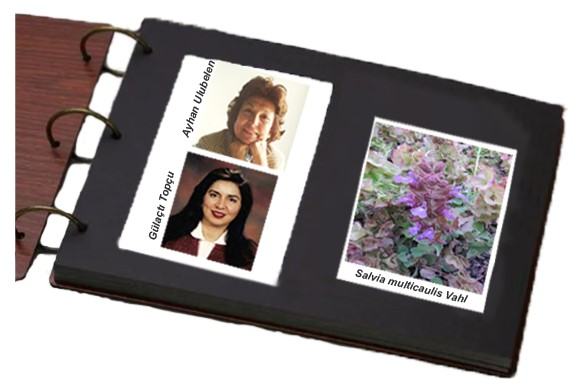
\includegraphics[width=12cm]{./pic/t1-1.jpg}
\end{figure}

在一篇关于\emph{Salvia multicaulis}Vahl.的研究中,Ulubelen和Topçu分离出了4种具有抗结核活性的全新芳香松香烷型二萜\textbf{1}--\textbf{4}。不仅分离出的二萜化合物具有抗细菌和抗真菌活性,植物提取物也显示出抗氧化、消炎和抑制胆碱酯酶的活性。\emph{S. multicaulis}在小亚细亚民间亦有使用,如作为开胃菜、用于促进伤口愈合,以及治疗蝎子叮咬、呼吸道感染、尿路感染和糖尿病等。

\begin{figure}[h]
	\centering
	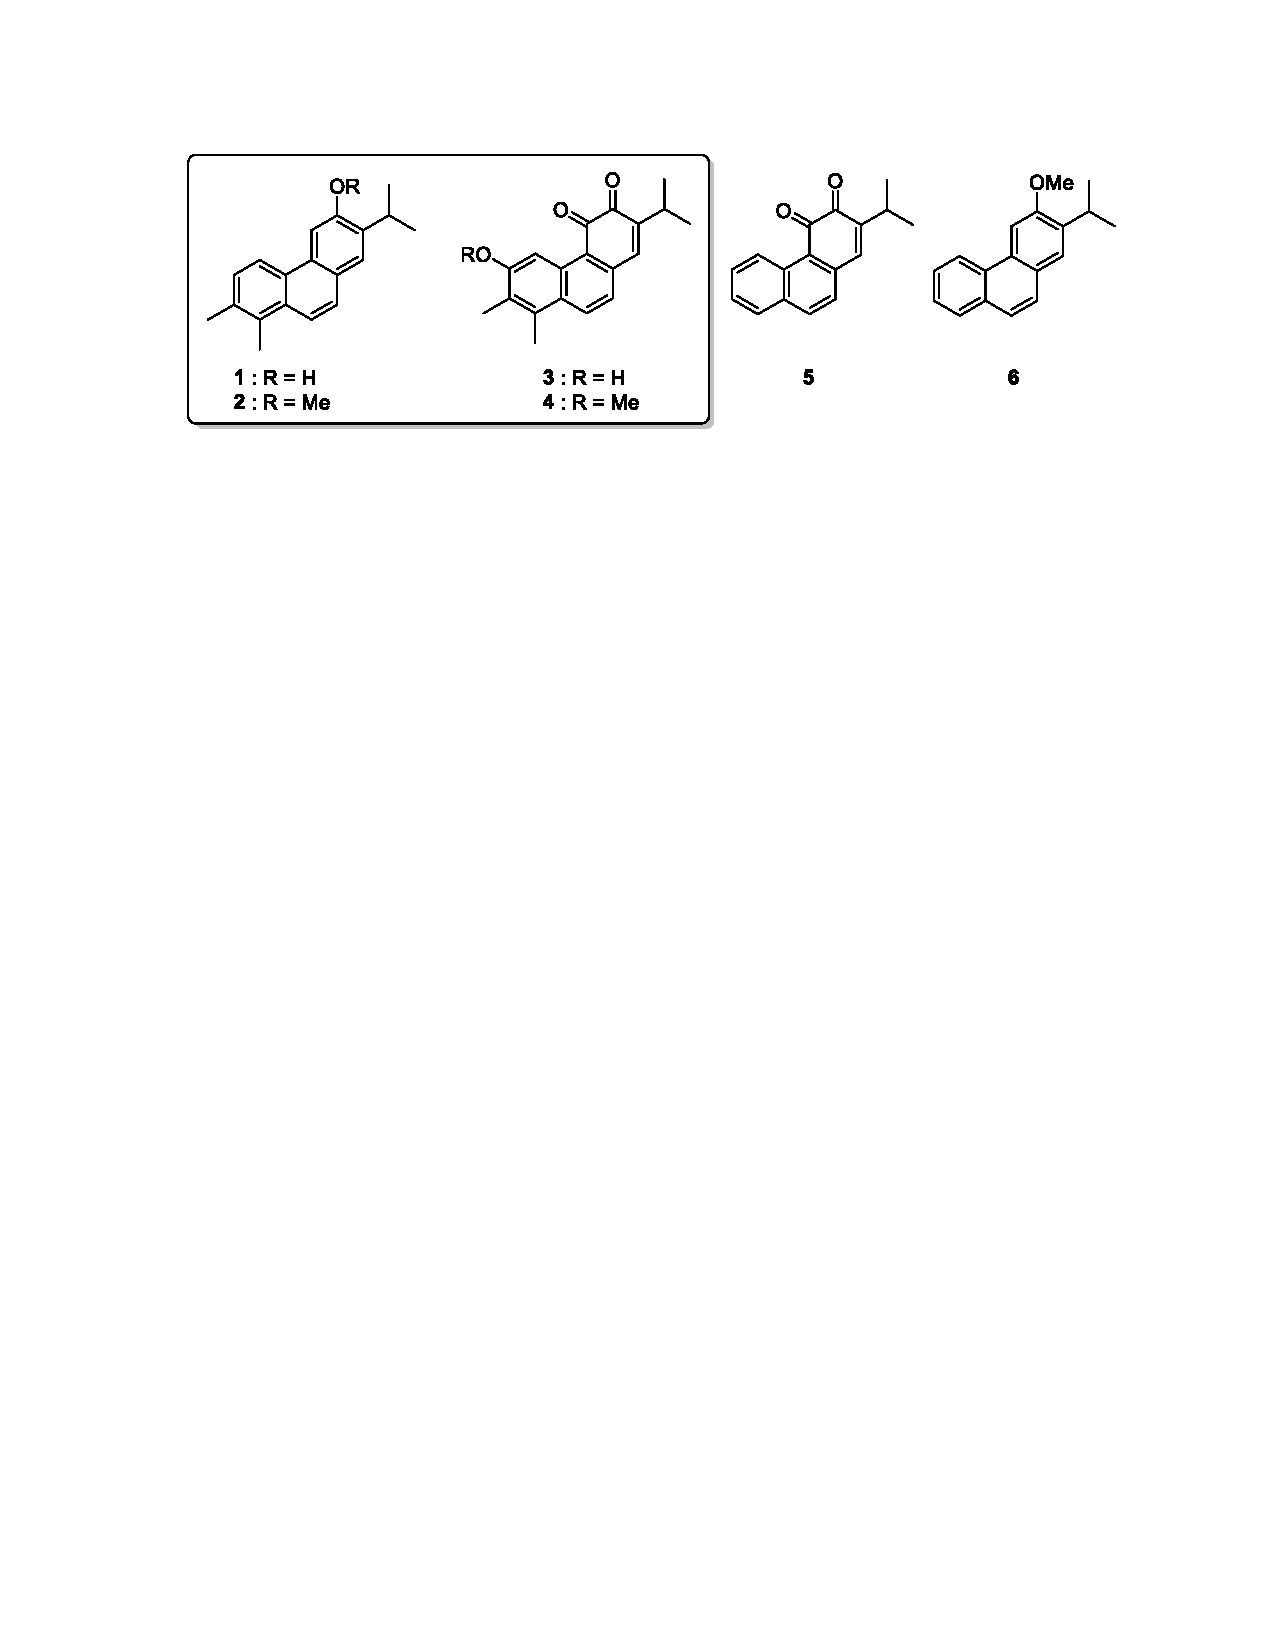
\includegraphics[width=14cm]{./pic/t1-2.pdf}
\end{figure}

随后一个土耳其的研究组发展了天然产物\textbf{1}--\textbf{4}衍生物的合成路线,本题就来源于此。合成二萜\textbf{1}和\textbf{5}的反应图如下所示。

\begin{figure}[h]
	\centering
	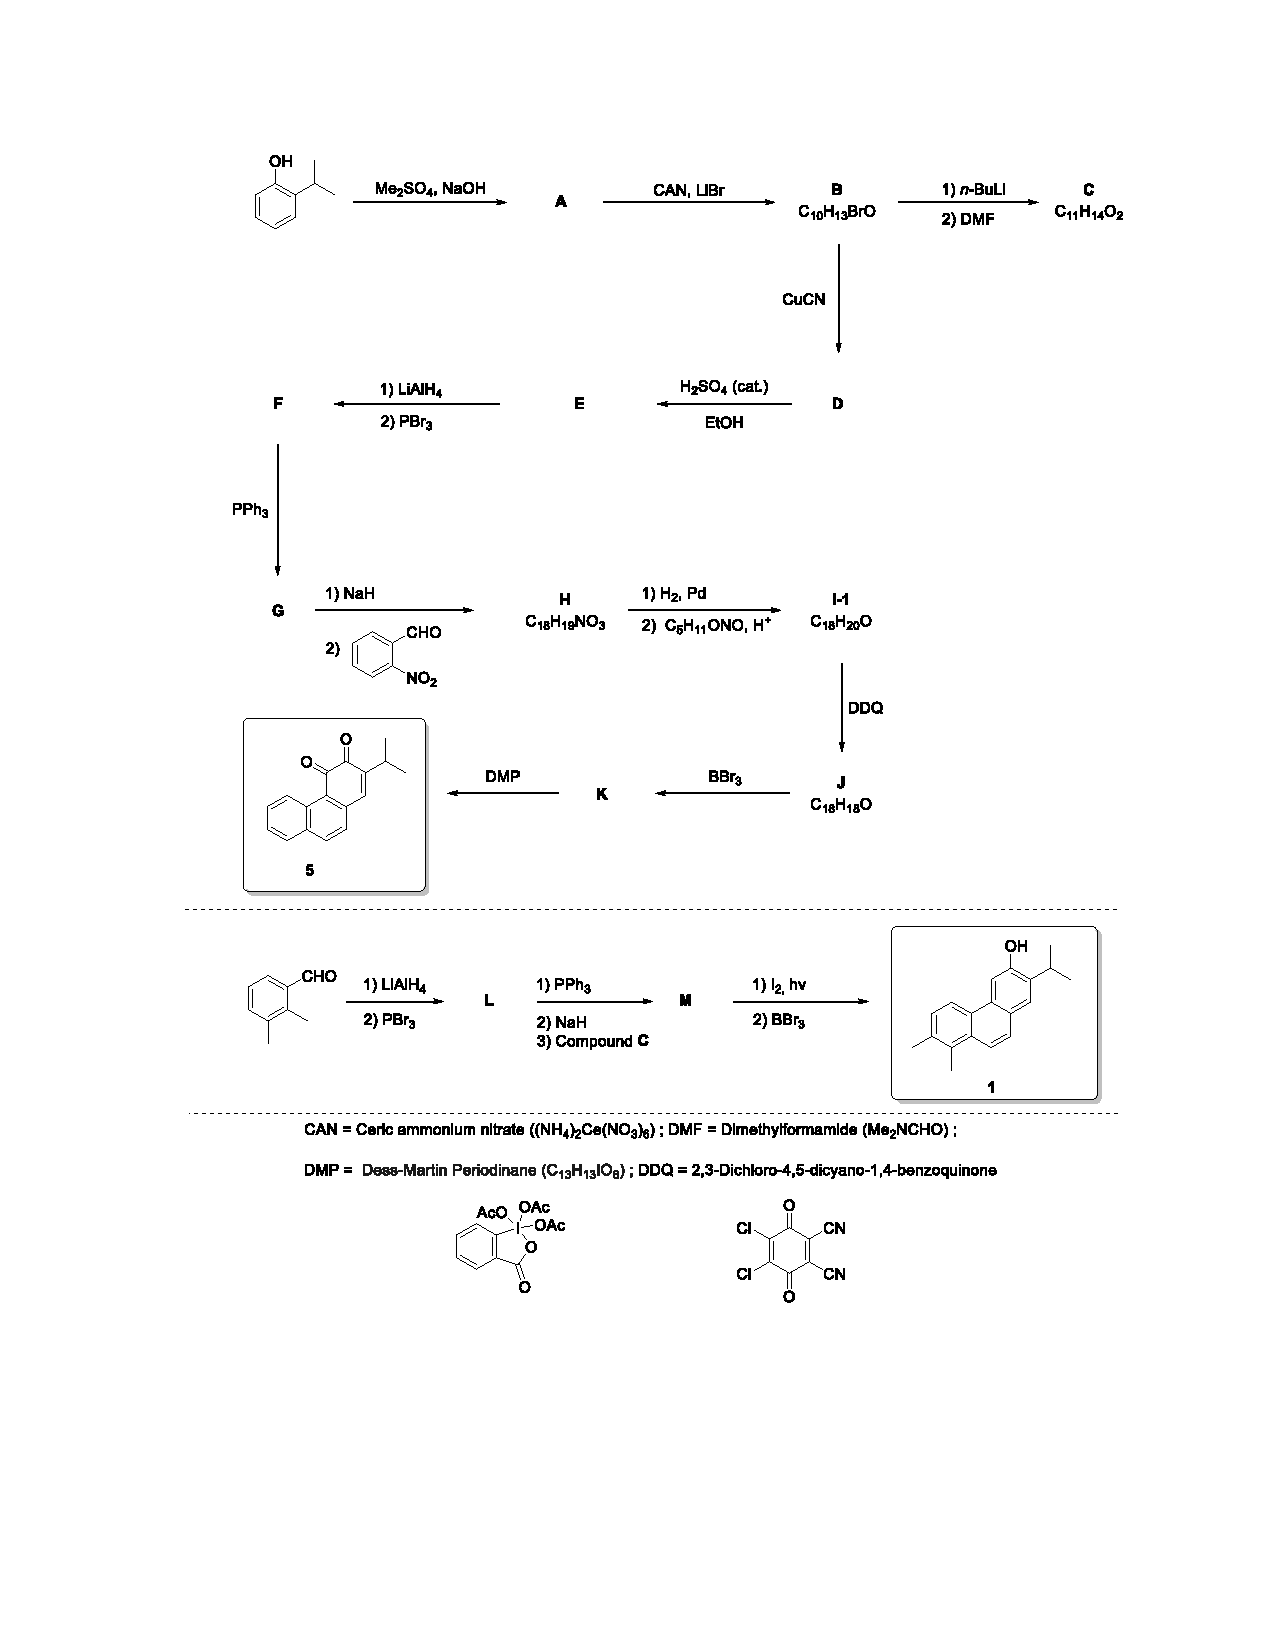
\includegraphics[width=16cm]{./pic/t1-3.pdf}
\end{figure}

\noindent\textbf{1.1.} 画出产物\textbf{A}--\textbf{M}的结构,无需考虑立体构型。\textbf{提示}:第二步 (\textbf{A}$\rightarrow$\textbf{B})中,溴化锂和硫酸铈(IV)铵合用作溴化试剂。化合物\textbf{C}是苯甲醛衍生物并用于化合物\textbf{M}的多步合成中。

\noindent\textbf{1.2.}\textbf{H}到\textbf{I1}的环化过程中同时生成了异构体\textbf{I2},其化学式为C\textsubscript{18}H\textsubscript{20}O。画出\textbf{I2}的结构。

\noindent\textbf{1.3.} 接下来的反应图与二萜\textbf{1}和\textbf{2}的去甲基衍生物\textbf{6}有关。画出产物\textbf{N}--\textbf{Y},无需考虑立体构型。\textbf{提示}:化合物\textbf{R}、\textbf{S}、\textbf{T}有酸性。化合物\textbf{V}到\textbf{W}的转化包含Robinson增环和一个可能的去甲酰化过程。

\noindent\textbf{1.4.} 化合物\textbf{V}到\textbf{W}的转化过程中,使用$\alpha$,$\beta$--不饱和酮的前体(例如$\beta$--氯代酮或\emph{N},\emph{N},\emph{N}--三烷基--3--氧代丁基卤化铵)更好。解释原因。

\noindent\textbf{1.5.} 画出化合物\textbf{V}可能的异构体。

\noindent\textbf{1.6.} 化合物\textbf{Y}也可由化合物\textbf{Z}经电环化关环得到。画出\textbf{Z}的结构。

\noindent\textbf{1.7.} 从\textbf{X}到\textbf{Y}的转化也可使用下列哪组试剂?(忽略S\textsubscript{N}2$'$反应)。

\begin{figure}[h]
	\centering
	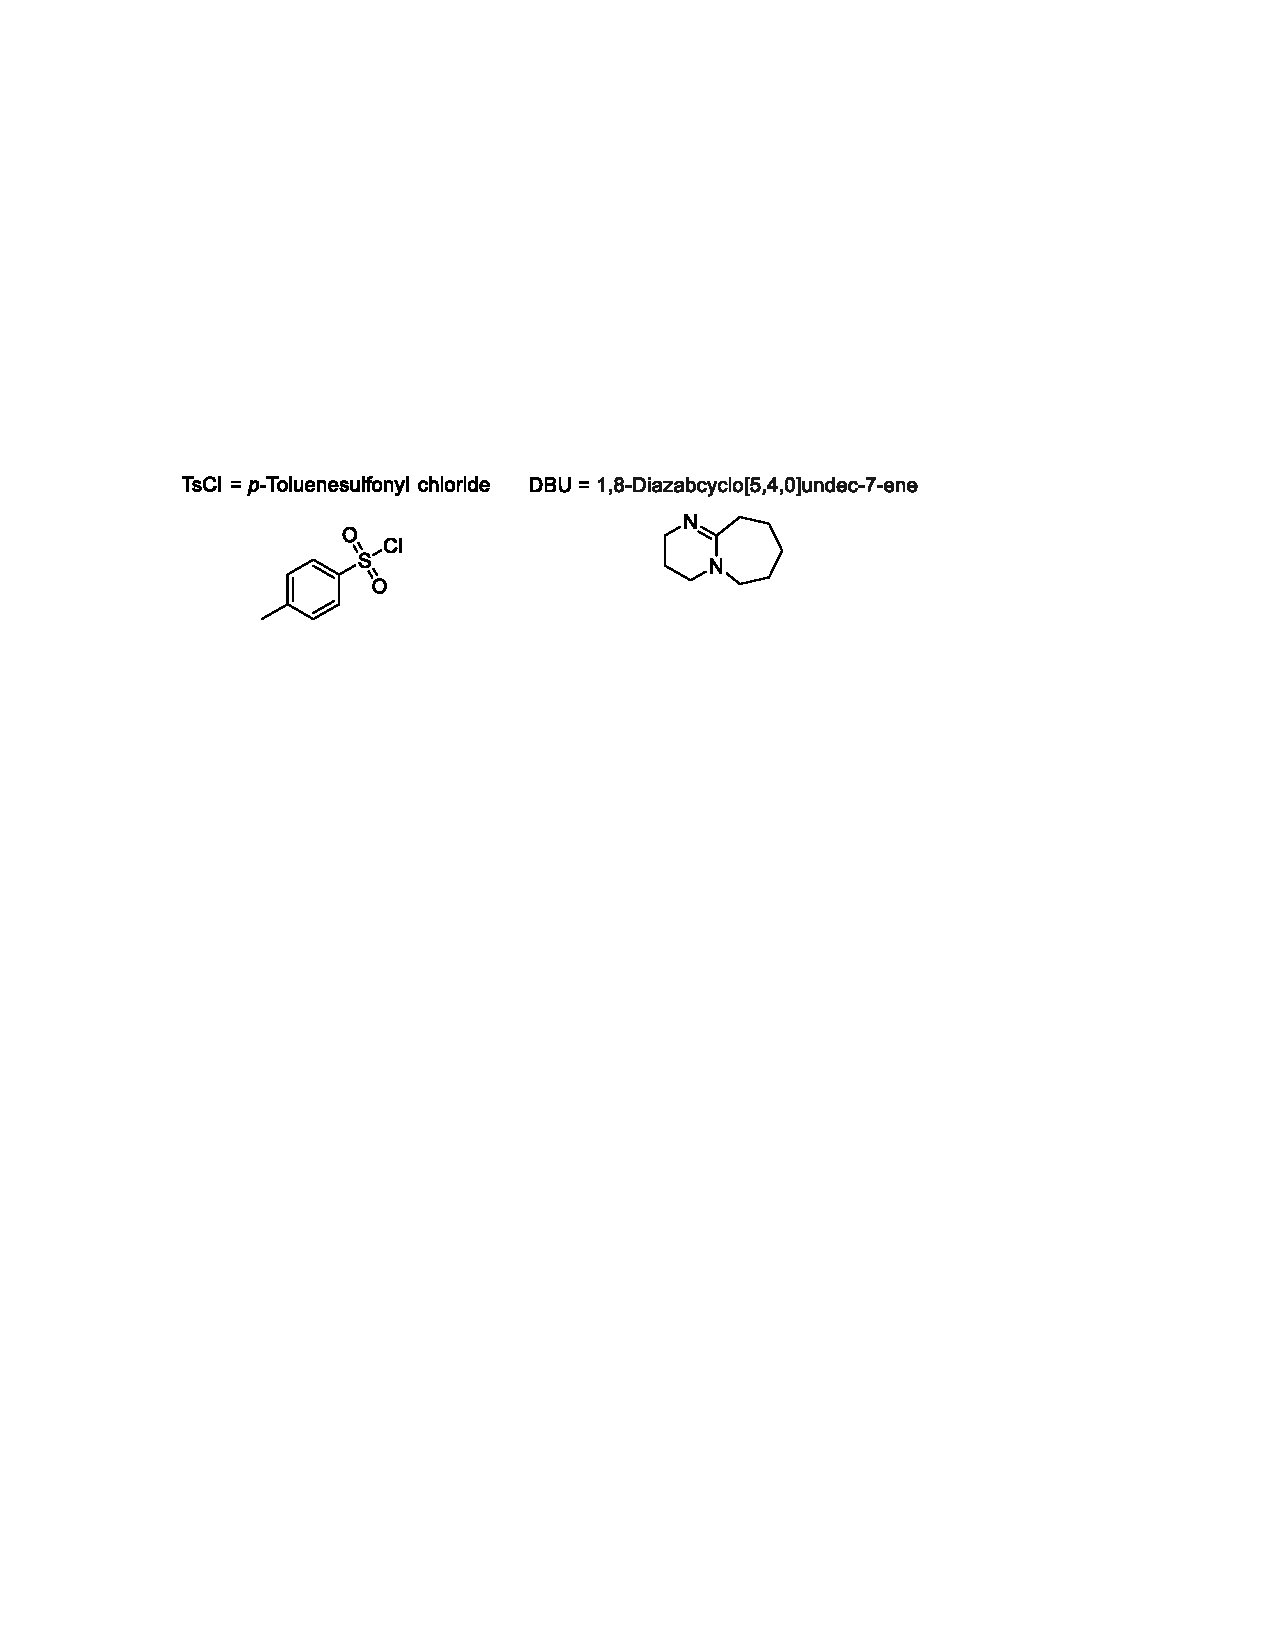
\includegraphics[width=12cm]{./pic/t1-5.pdf}
\end{figure}

\renewcommand{\labelitemi}{$\square$}
\begin{itemize}
	\item i) PBr\textsubscript{3}/吡啶; ii)  \textit{n}--Bu\textsubscript{3}SnH/AIBN
	\item i) PBr\textsubscript{3}/吡啶; ii) Na/\emph{t}--BuOH
	\item i) MnO\textsubscript{2}; ii) DDQ
	\item i) TsCl/吡啶; ii) LiAlH\textsubscript{4}
	\item TsCl/吡啶; ii) DBU
\end{itemize}
\renewcommand{\labelitemi}{$\bullet$}

\begin{figure}[h]
	\centering
	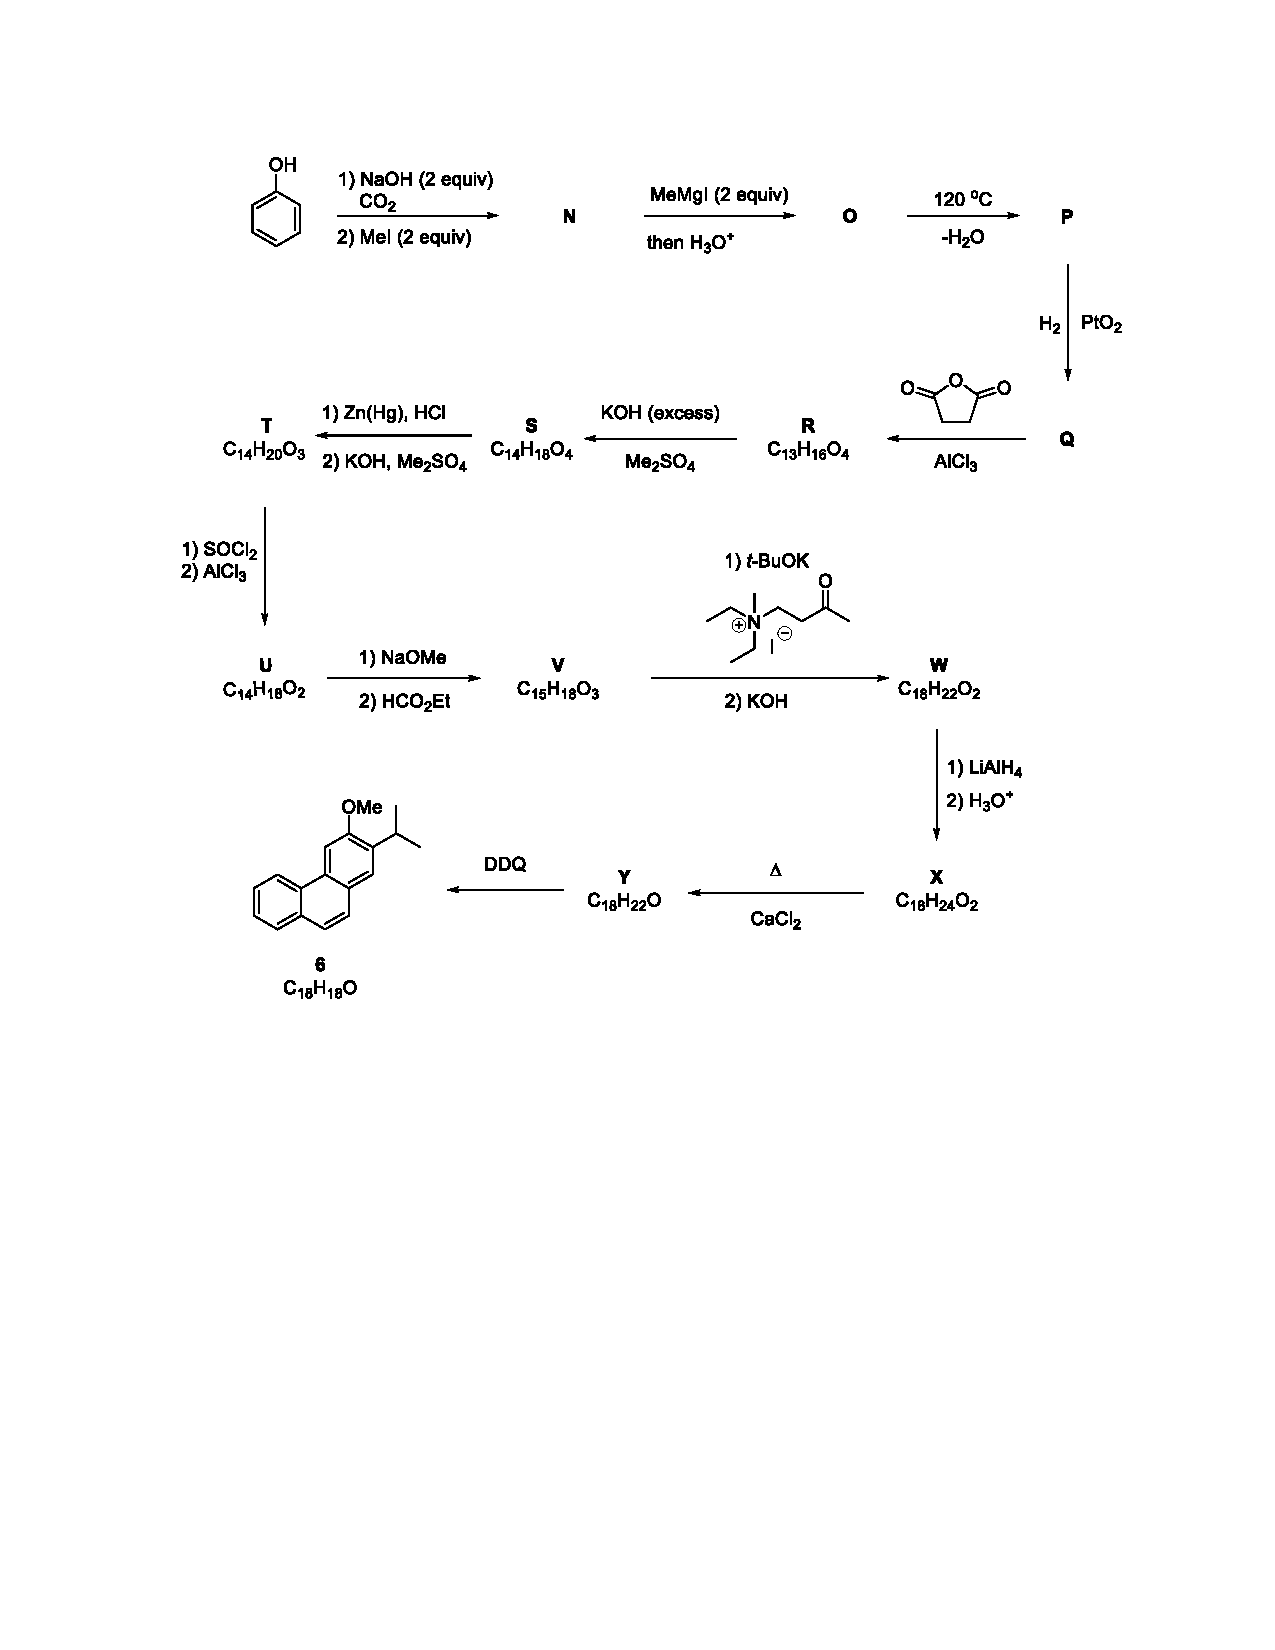
\includegraphics[width=15cm]{./pic/t1-4.pdf}
\end{figure}

\newpage
\mysection{第2题\  Istanbulin和相关的倍半萜天然产物}
\textbf{图}

一些元素的名字源于由世界各地的地名。这一点上,瑞典村庄Ytterby创造了一项纪录,四种元素:镱(ytterbium,Yb)、钇(yttrium,Y)、铒(erbium,Er)和铽(terbium,Tb)得名于此。然而,并不仅仅是元素会以地名命名。有趣的是,一系列天然产物\textbf{istanbulin A--E}的名字源于城市伊斯坦布尔。这一系列的前两个成员即istanbulin A和B首次于1971年由教授Ayhan Ulubelen博士及其合作者从植物\emph{Smyrnium olusatrum}(译注:又名亚历山大草)中分离得到。剩下的3个成员即istanbulin C--E由Ulubelen及其合作者在1979年至1982年间报道。

\textbf{图}

Istanbulin是倍半萜天然产物这一更大家庭中的一员。Vernolepin \textbf{1}和vernomenin \textbf{2}是两种重要的倍半萜天然产物,它们具有类似的6-6-5并环体系。1976年,Danishefsky及其合作者报道了这两个化合物的全合成。在这一漂亮的全合成路线中,Danishefsky将所谓Danishefsky二烯用于Diels--Alder (DA)反应中。

请注意本题中所有的手性化合物的结构式都表示外消旋体。

\textbf{图}

上下文中提到的Danishefsky二烯 \textbf{3}和Rawal--Kozmin二烯 \textbf{4}是两个富电子二烯,都已广泛用于有机合成中。它们的结构如下所示:

\textbf{图}

TMS: 三甲基硅基;TBS: 叔丁二甲基硅基

\noindent\textbf{2.1.}画出\textbf{3}和\textbf{4}主要的共振式。指出每个二烯中电子密度最高的碳原子。

\noindent\textbf{2.2.}化合物\textbf{3}和\textbf{4}广泛用作Diels--Alder反应的双烯体。画出\textbf{3}和\textbf{4}能够发生DA反应时的构象。推测在与顺丁烯二酸酐发生DA反应时,哪个二烯的活性更高?

加热Danishefsky二烯 \textbf{3}与化合物\textbf{6}的混合物,随后用酸(TsOH,对甲苯磺酸)处理,得到主要产物化合物\textbf{A}。

\noindent\textbf{2.3.}画出\textbf{3}和\textbf{6}发生Diels--Alder反应所有可能的产物,它们的化学式都为C\textsubscript{12}H\textsubscript{14}O\textsubscript{3}。每一组对映异构体画出其中一种即可。

\textbf{图}

\noindent\textbf{2.4.} 确定主产物\textbf{A}的结构。

\noindent\textbf{2.5.} Diels--Alder加合物\textbf{A}依次经历如下的4步反应转化为化合物\textbf{7}。化合物\textbf{B}具有酸性。画出\textbf{B}-\textbf{D}的结构。

\textbf{图}

\noindent\textbf{2.6.} 化合物\textbf{7}与1当量\emph{m}-CPBA反应得到主产物\textbf{E}。圈出与\emph{m}-CPBA选择性发生反应的官能团,画出\textbf{E}的结构。

\noindent\textbf{2.7.} Vernolepin \textbf{1} 和 vernomenin \textbf{2}的全合成经如下步骤完成。画出化合物\textbf{F}-\textbf{J}的结构。最后一步中,化合物\textbf{I}是\textbf{1}的前体。

\textbf{图}

\newpage
\mysection{第3题\  茶,荼,檟,蔎,茗,荈和格雷伯爵茶之味:香柠檬}
一曰茶,二曰檟,三曰蔎,四曰茗,五曰荈

\begin{flushright}
------陆羽 《茶经》
\end{flushright}

茶(土耳其语:çay)流行于土耳其以及海外土耳其人中。土耳其茶文化同时影响了阿塞拜疆在内的巴尔干半岛诸国。土耳其的人均茶消耗量世界第一,达到2.5
kg/人/年,紧随其后的是英国(2.1 kg/人/年)。

香柠檬烯(bergamotene)及其衍生物\textbf{1}-\textbf{4}属倍半萜类化合物,皆为蒎烷类单萜的类似物。香柠檬烯存在于香柠檬油中,是格雷伯爵茶香和味的来源。

\begin{figure}[h]
	\centering
	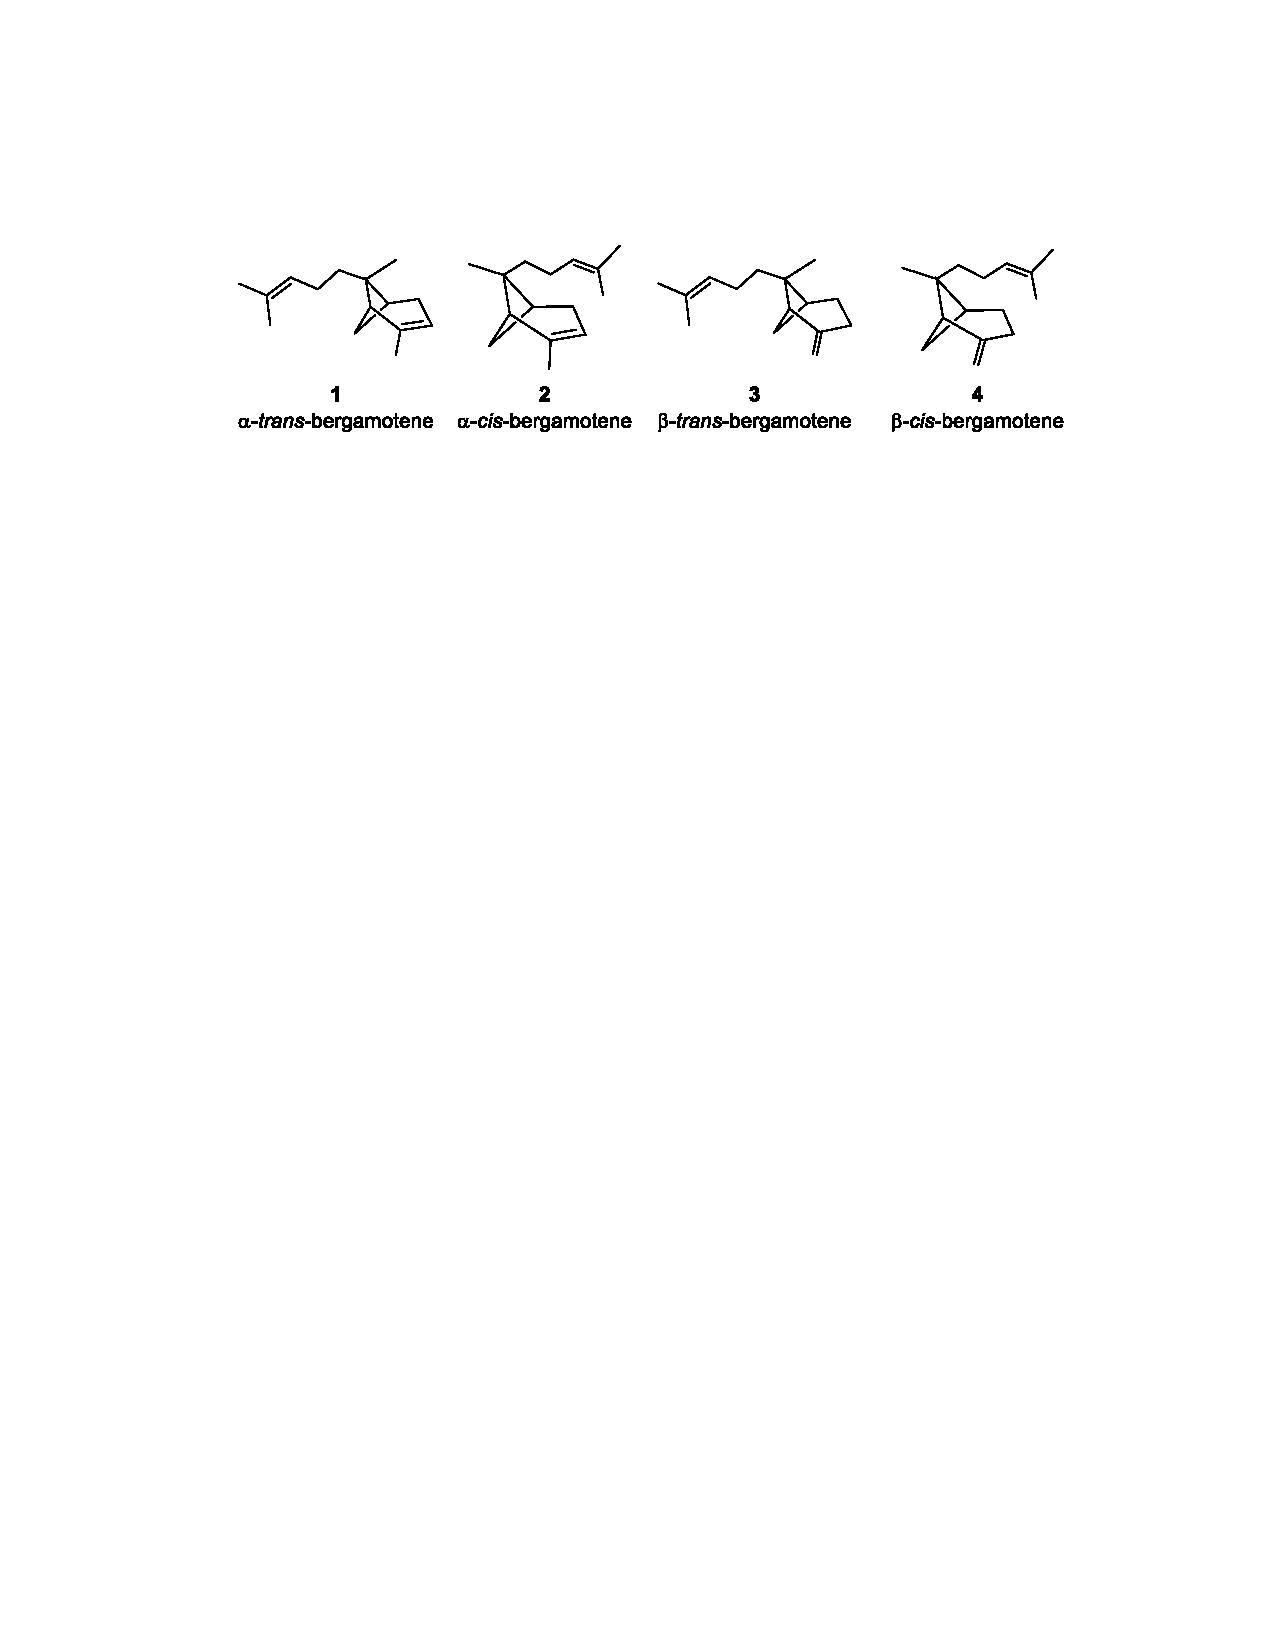
\includegraphics[width=13cm]{./pic/t3-1.pdf}
\end{figure}

\noindent\textbf{3.1.}以下的反应图示出了$\alpha$-反式香柠檬烯\textbf{1}的合成路线。画出产物\textbf{A}-\textbf{G}的结构。

\noindent\textbf{3.2.} 从\textbf{A}到\textbf{B}的转化中,试剂Me\textsubscript{3}NO的作用是什么?

\begin{figure}[h]
	\centering
	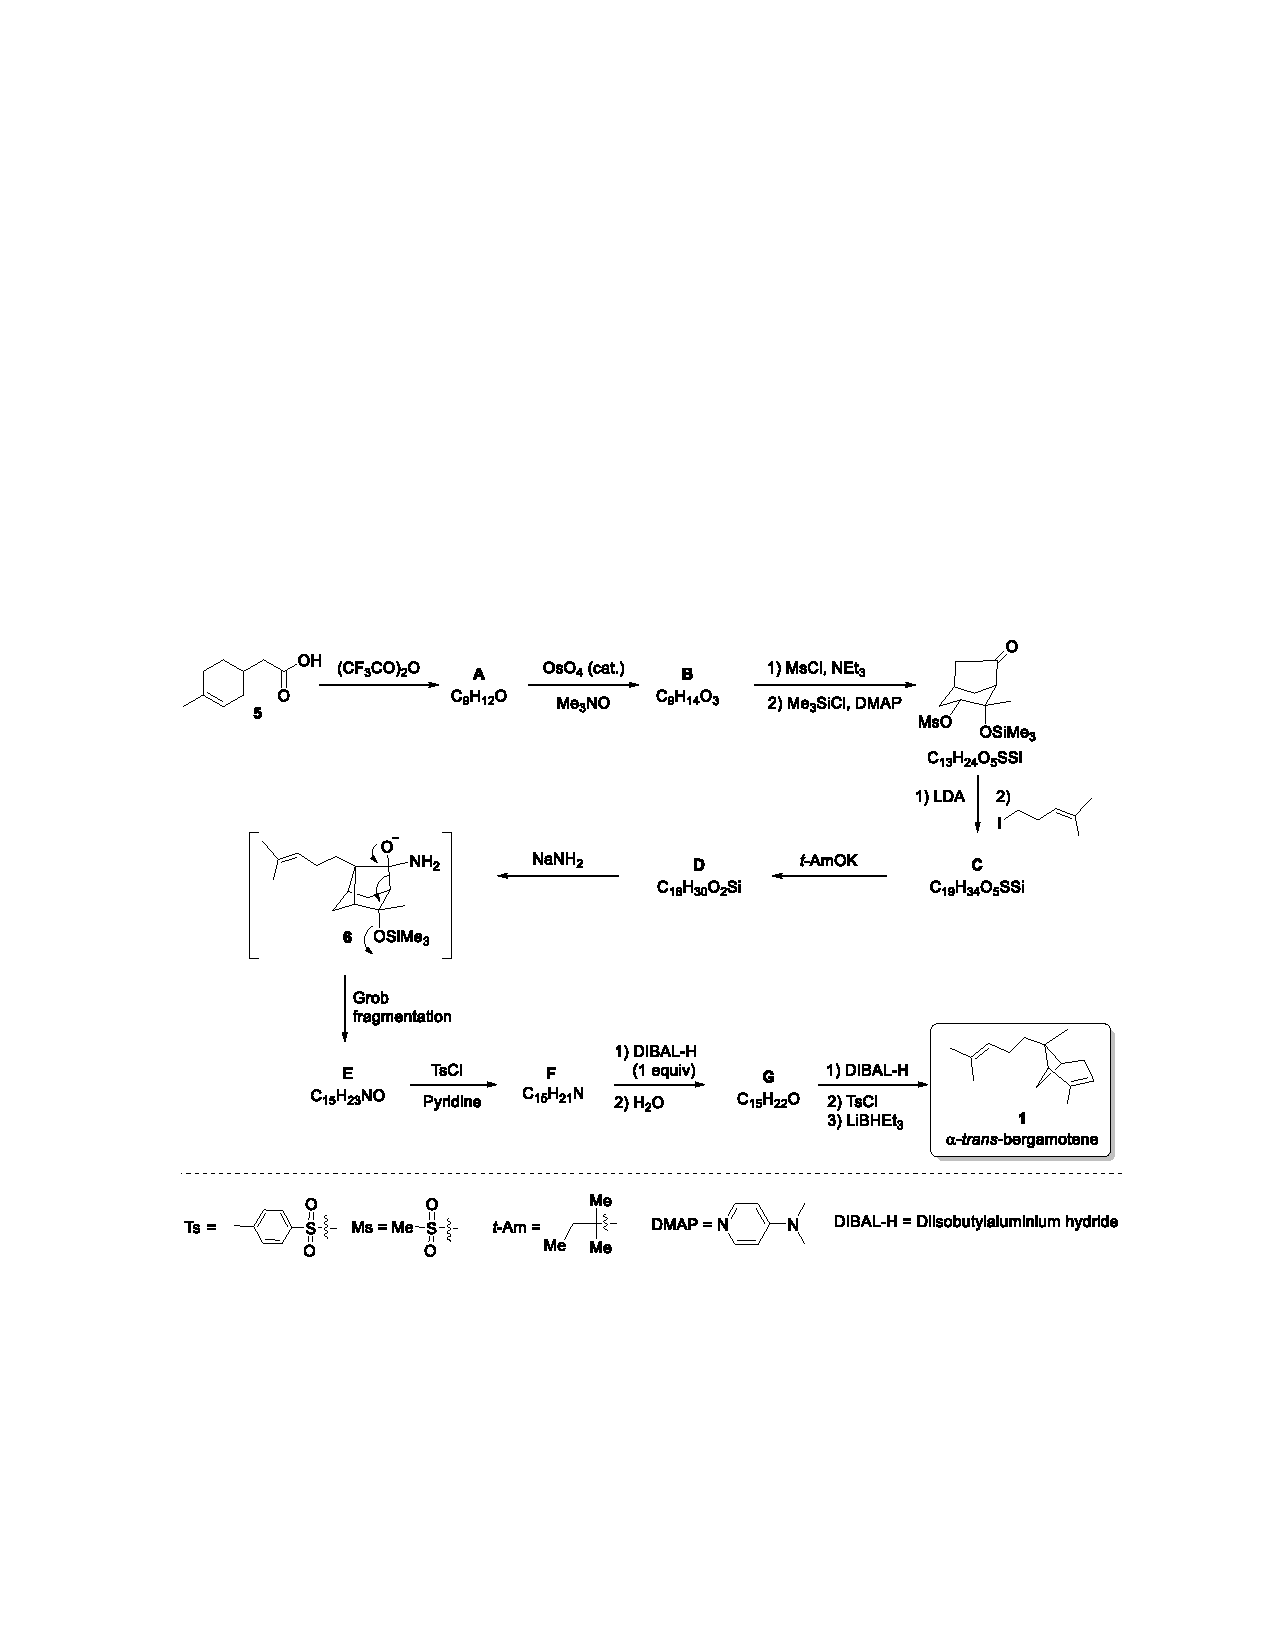
\includegraphics[width=16cm]{./pic/t3-2.pdf}
\end{figure}


\newpage
\mysection{第14题\  抗癌的铂络合物}
\begin{figure}[h]
	\centering
	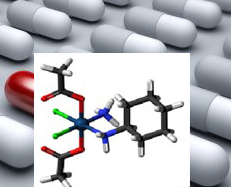
\includegraphics[width=7cm]{./pic/t14-1.png}
\end{figure}

基于金属药物的药用无机化学被广泛定义为与金属离子和金属络合物及其临床应用有关的研究领域。这是从抗癌药顺铂的发现发展起来的一个新的研究领域。顺铂,顺二氯二氨铂(II),是一种黄色粉末,也是一种抗癌药物。其广泛用于治疗多种肿瘤,尤其是睾丸,卵巢,头和颈部的肿瘤。

顺铂的合成始于K\textsubscript{2}[PtCl\textsubscript{4}],自100多年前发表以来,已经历了几处改进。主要问题是杂质的出现和副产物反铂的形成。如今合成路线主要基于Dhara在1970年代发表的方法。在初始步骤中,K\textsubscript{2}[PtCl\textsubscript{4}]与过量的KI反应,然后将铂络合物转化为碘类似物\textbf{A}。随后,将NH\textsubscript{3}加入化合物\textbf{A}中,并通过配体交换形成化合物\textbf{B},其中两个NH\textsubscript{3}配体与两个碘配体交换。\textbf{B}是黄色固体,将其过滤,干燥并与AgNO\textsubscript{3}的水溶液混合。可以滤出不溶的AgI,形成顺式二氨二水合铂硝酸盐\textbf{C};然后将过量的KCl加入\textbf{C}溶液中,得到顺铂\textbf{D}。

合成的成功取决于碘配体的强反位效应。在平面四方配合物中与离去基团处在反式的旁观配体\textbf{T}影响取代的速度。这种现象称为反位效应。关键是强的$\sigma$给体配体或$\pi$受体配体极大地促进了反式的配体取代。反位效应遵循以下顺序。

作为$\sigma$给体的\textbf{T}:OH\textsuperscript{−}< NH\textsubscript{3}<Cl\textsuperscript{−}<Br\textsuperscript{−}<CN\textsuperscript{−},CH\textsubscript{3}\textsuperscript{−}<I\textsuperscript{−}<SCN\textsuperscript{−},PR\textsubscript{3},H\textsuperscript{−}

对于$\pi$受体的\textbf{T}:Br\textsuperscript{‑}<I\textsuperscript{−}<NCS\textsuperscript{−}<NO\textsubscript{2}\textsuperscript{−}<CN\textsuperscript{−}<CO,C\textsubscript{2}H\textsubscript{4}

\begin{figure}[h]
	\centering
	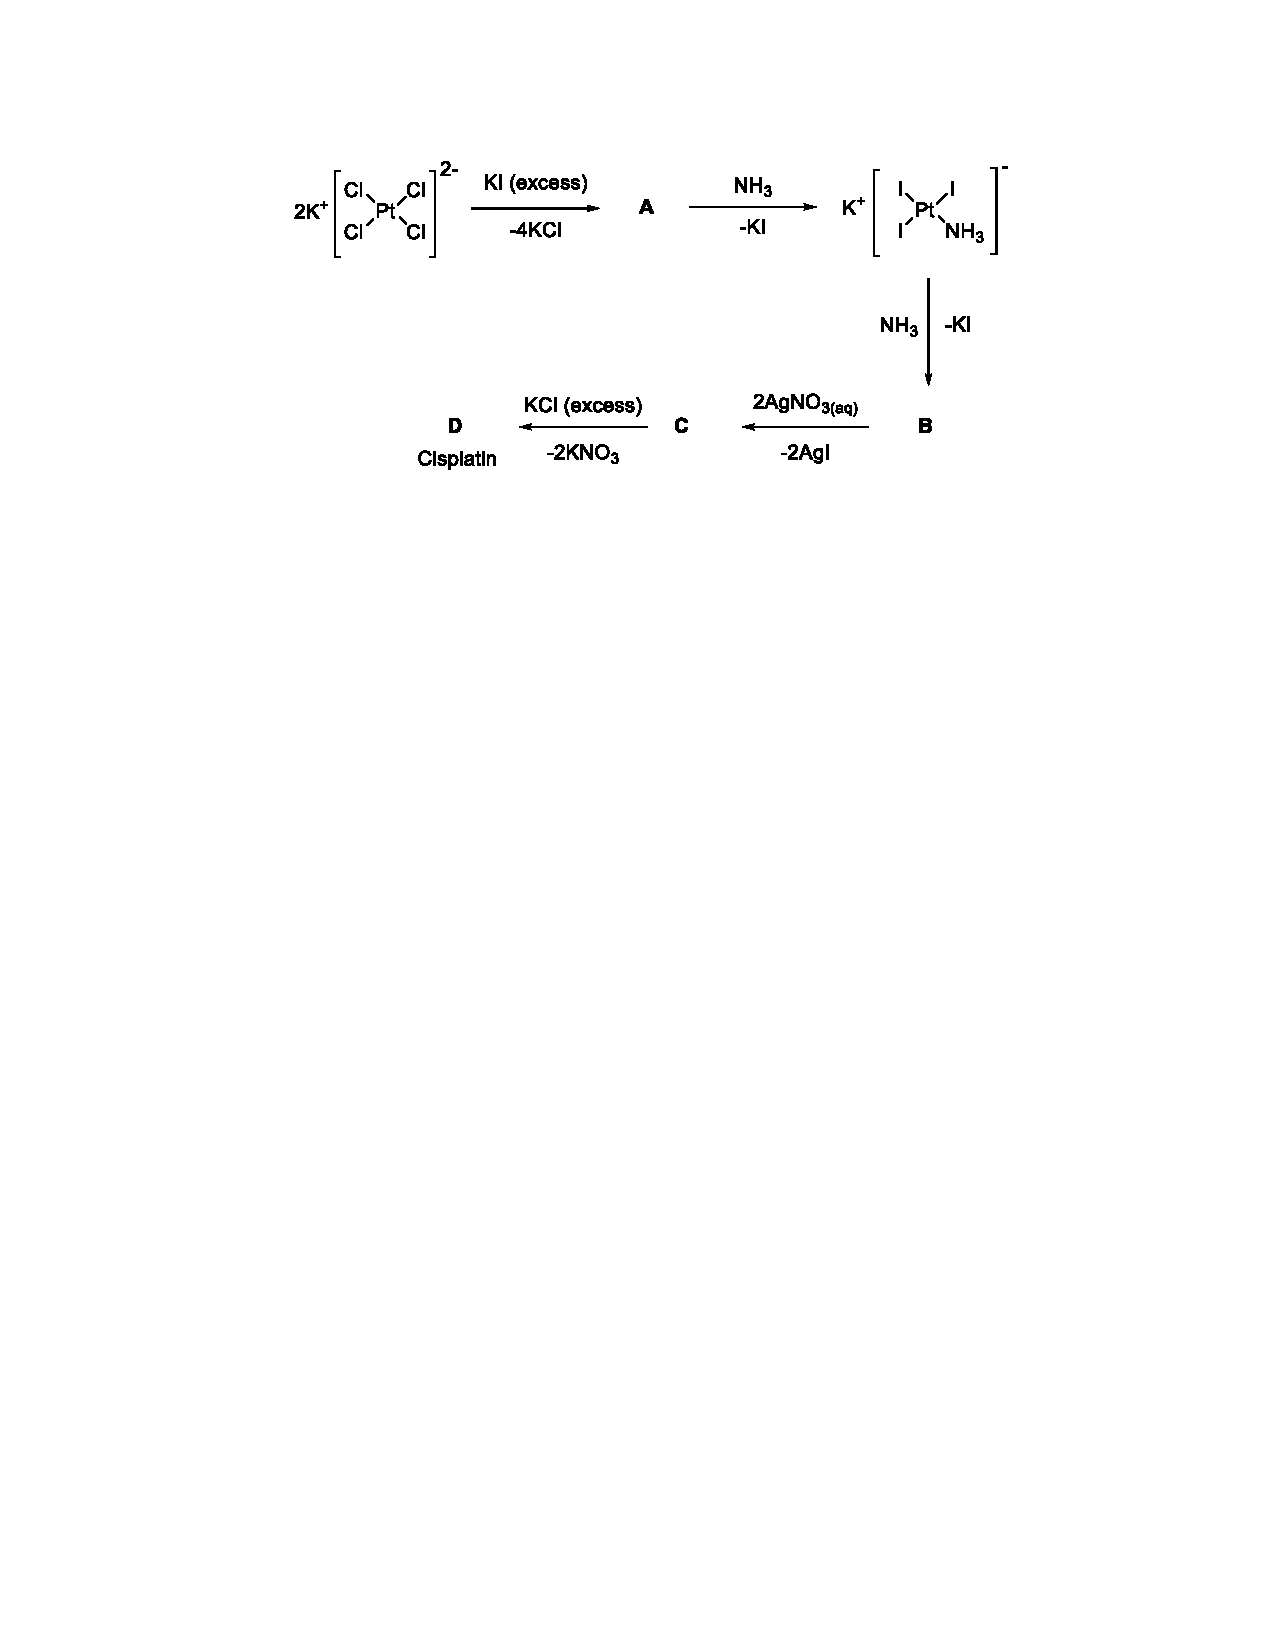
\includegraphics[width=13cm]{./pic/t14-2.pdf}
\end{figure}

\noindent\textbf{14.1.} 写出\textbf{A}-\textbf{D}的分子式

\noindent\textbf{14.2.} 画出\textbf{A}-\textbf{D}的分子结构

\noindent\textbf{14.3.} 化合物\textbf{D}是极性的吗?

\noindent\textbf{14.4.} 运用晶体场理论,画出顺铂\textbf{D}的\textit{d}轨道分裂图并展示电子分配示意图。

\noindent\textbf{14.5.} 确定络合物\textbf{A}的磁性。

铂络合物与DNA结合并引起交联,从而触发程序性细胞死亡(细胞凋亡)。然而,平面四方结构的另一几何异构体反铂,反式二氯二氨合铂(II)\textbf{F},对癌症的治疗无效。反铂是从[Pt(NH\textsubscript{3})\textsubscript{4}]\textsuperscript{2+}开始合成的,然后陆续添加二个Cl\textsuperscript{−}配体以形成反铂\textbf{F},如下图所示。

\begin{figure}[h]
	\centering
	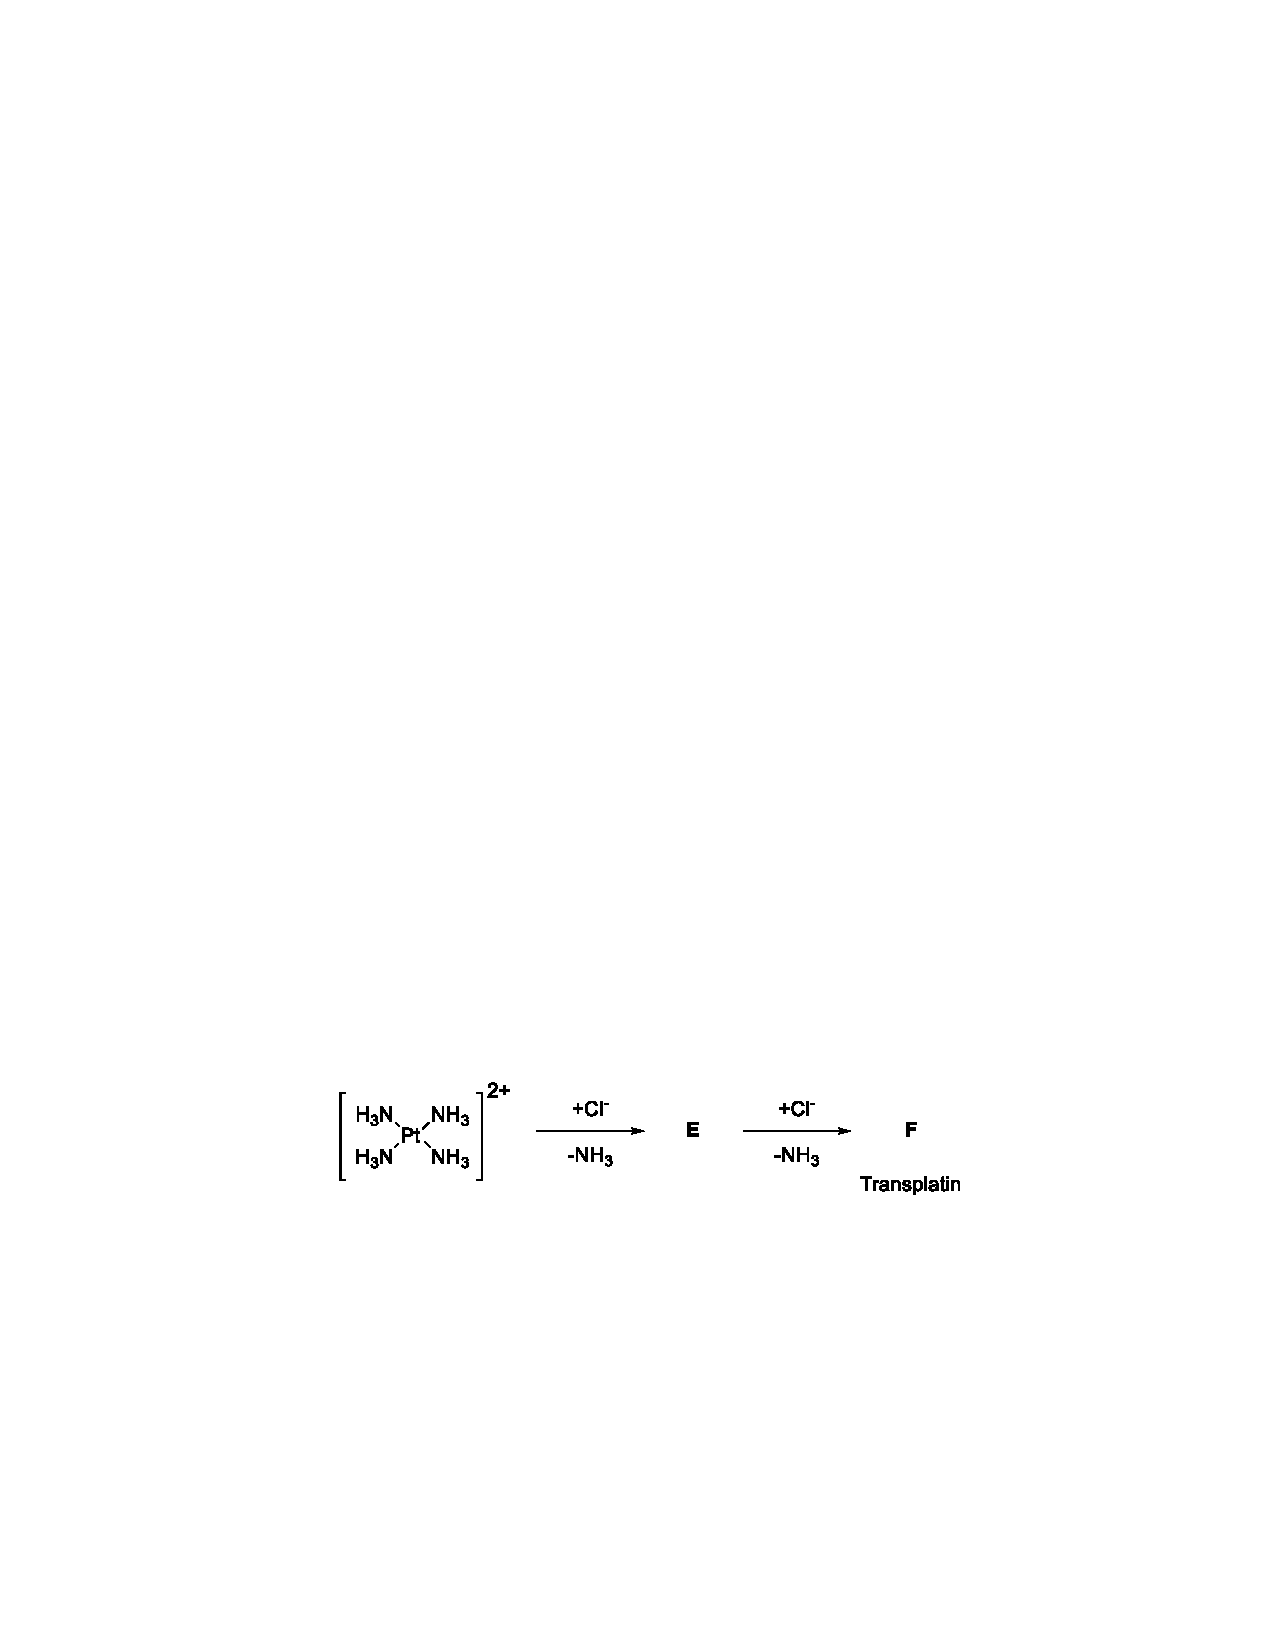
\includegraphics[width=11cm]{./pic/t14-3.pdf}
\end{figure}

\noindent\textbf{14.6.} 画出\textbf{E}和\textbf{F}的分子结构

最重要的一类抗肿瘤药顺铂,卡铂(carboplatin)和奥沙利铂(oxaliplatin)作为二胺合铂(II)被广泛用于化学疗法中,以治疗各种癌症。

\begin{figure}[h]
	\centering
	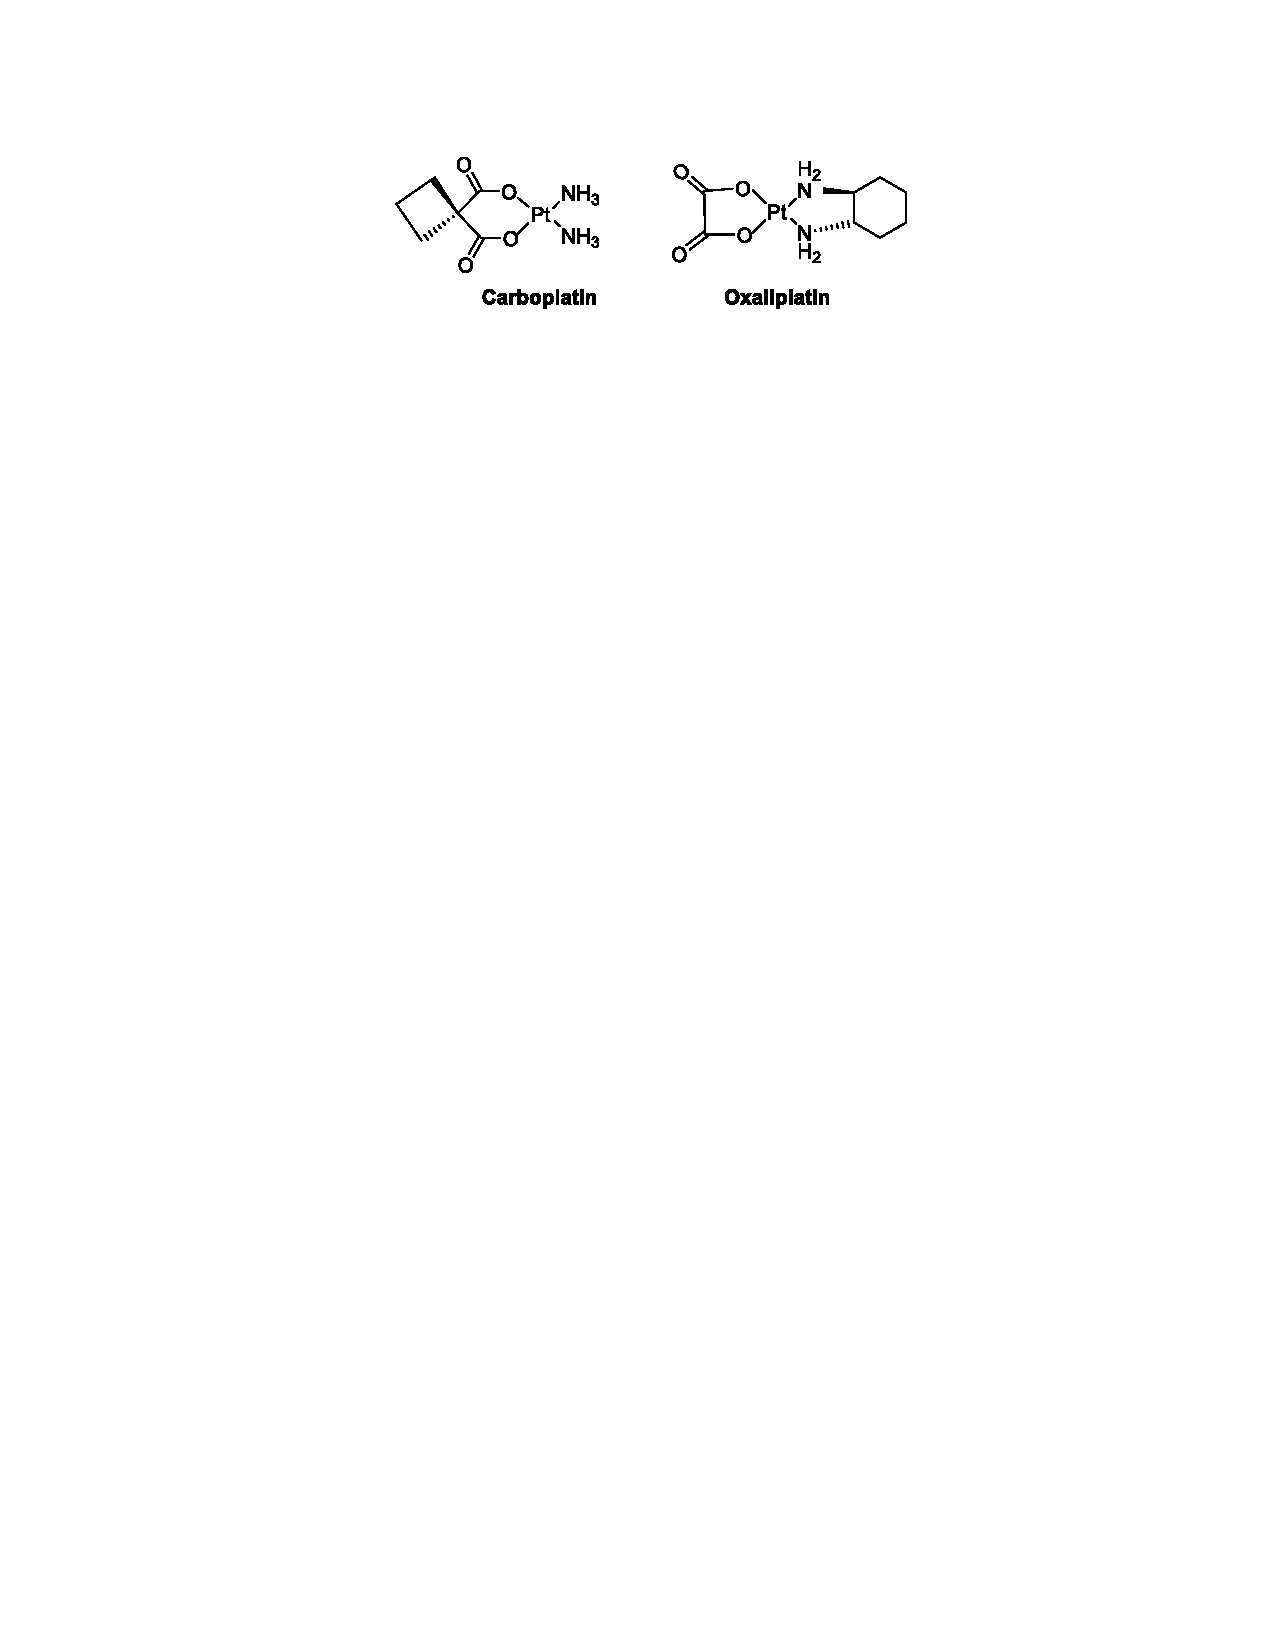
\includegraphics[width=8cm]{./pic/t14-4.pdf}
\end{figure}

但是,这些药物的治疗指数相对较窄。它们的使用经常受到严重毒性和抗药性的困扰,这导致疾病进展。最近,氧铂(oxoplatin),异丙铂(iproplatin),奥马铂(ormaplatin)和沙铂(satraplatin)是临床上已经使用的(氧铂)或试验中的铂络合物。

\begin{figure}[h]
	\centering
	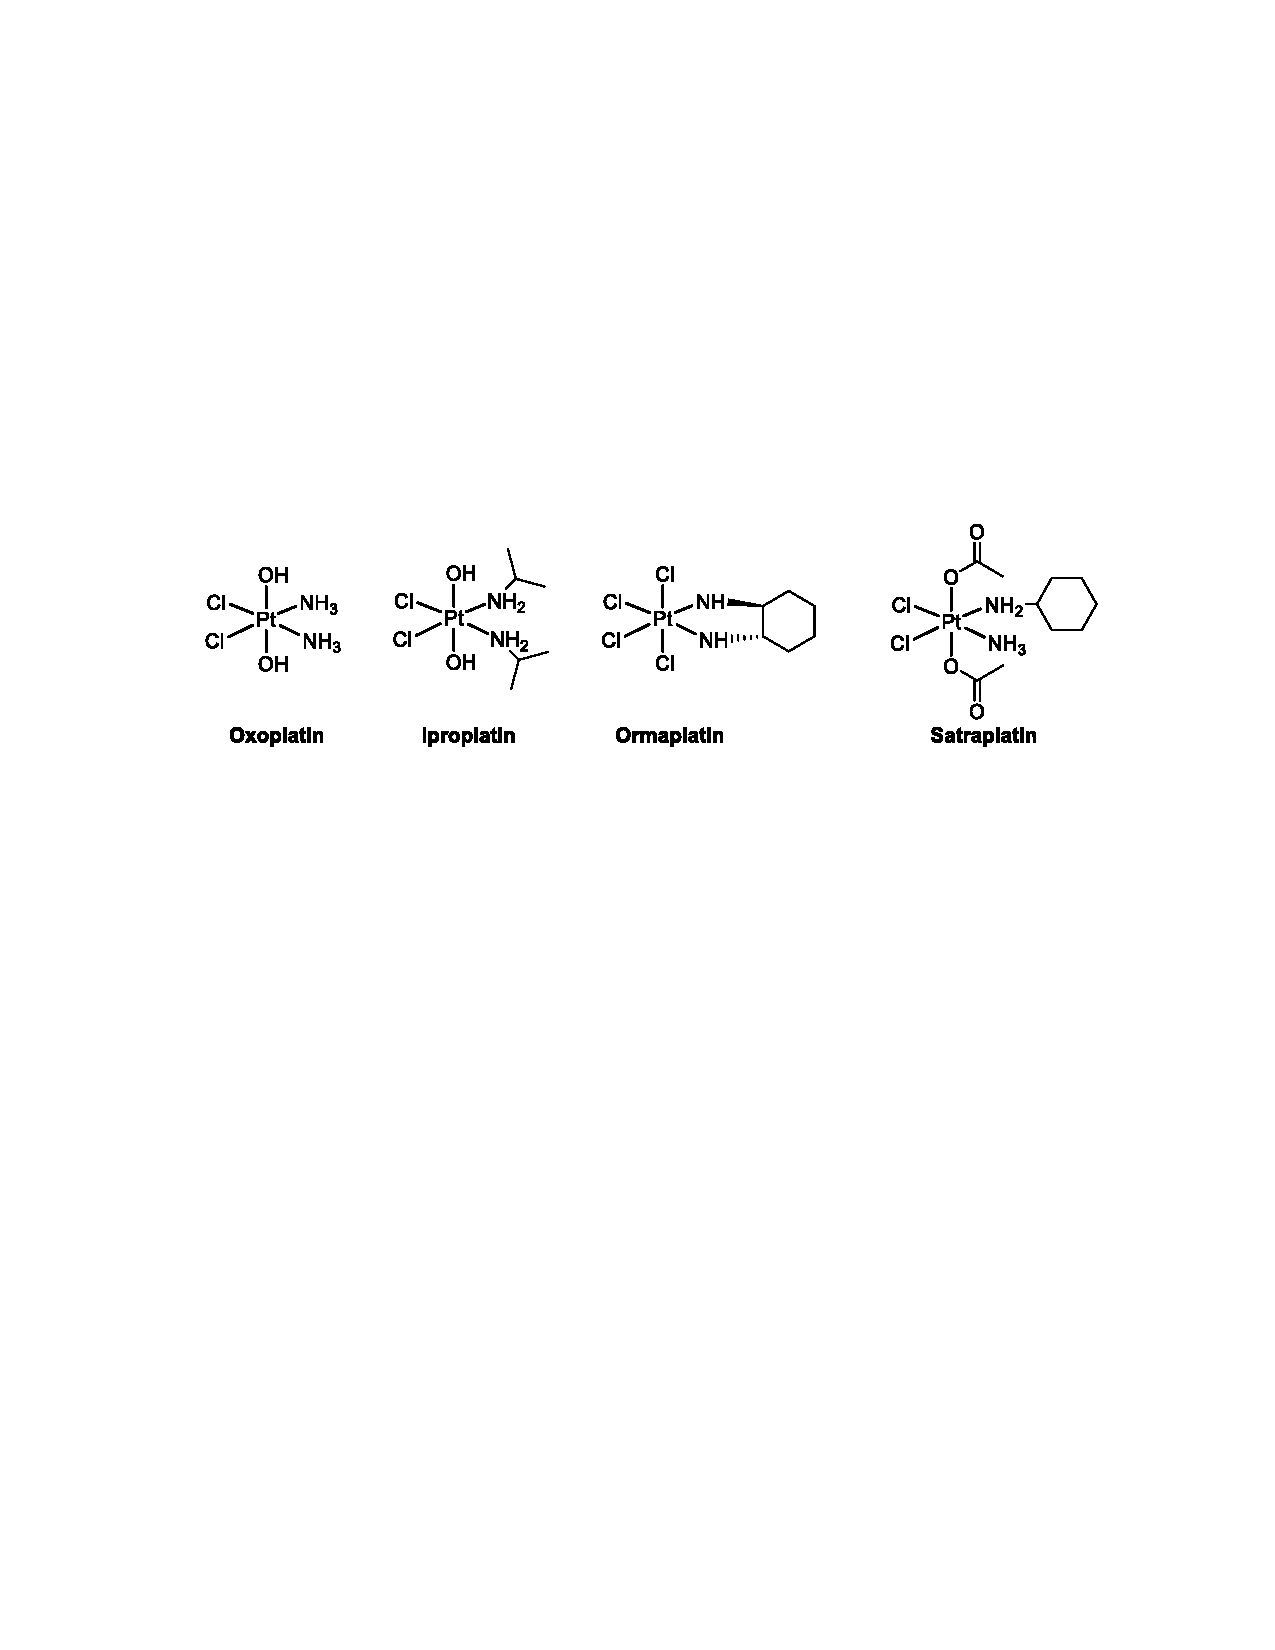
\includegraphics[width=13cm]{./pic/t14-5.pdf}
\end{figure}

\noindent\textbf{14.7.}
所有配合物有相同的几何结构和对于Pt中心原子的氧化数。写出Pt的氧化数和配合物的几何构型。

\noindent\textbf{14.8.} 哪一个Pt络合物,顺铂还是沙铂,对于取代反应更动力学惰性?

\noindent\textbf{14.9.}
奥沙铂是[Pt(NH\textsubscript{3})\textsubscript{2}Cl\textsubscript{2}(OH)\textsubscript{2}]的一个异构体。画出所有的立体异构体并指明哪些有手性。

铂络合物(氧铂,异丙铂,奥马铂和沙铂)可以被认为是前体药,其主要在细胞内被生物还原剂(如硫醇,抗坏血酸和谷胱甘肽(GSH))激活以杀死癌细胞。

例如,在一项研究中,癌细胞(A2780,A2780cisR和HT-29)的水溶液提取物可还原具有与沙铂相似结构的\textit{cis},\textit{trans},\textit{cis}-[PtCl\textsubscript{2}(OCOCH\textsubscript{3})\textsubscript{2}(NH\textsubscript{3})\textsubscript{2}](\textbf{G},前药)产生顺铂(\textbf{D},药物)和游离乙酸根离子,如下所示。

\begin{figure}[h]
	\centering
	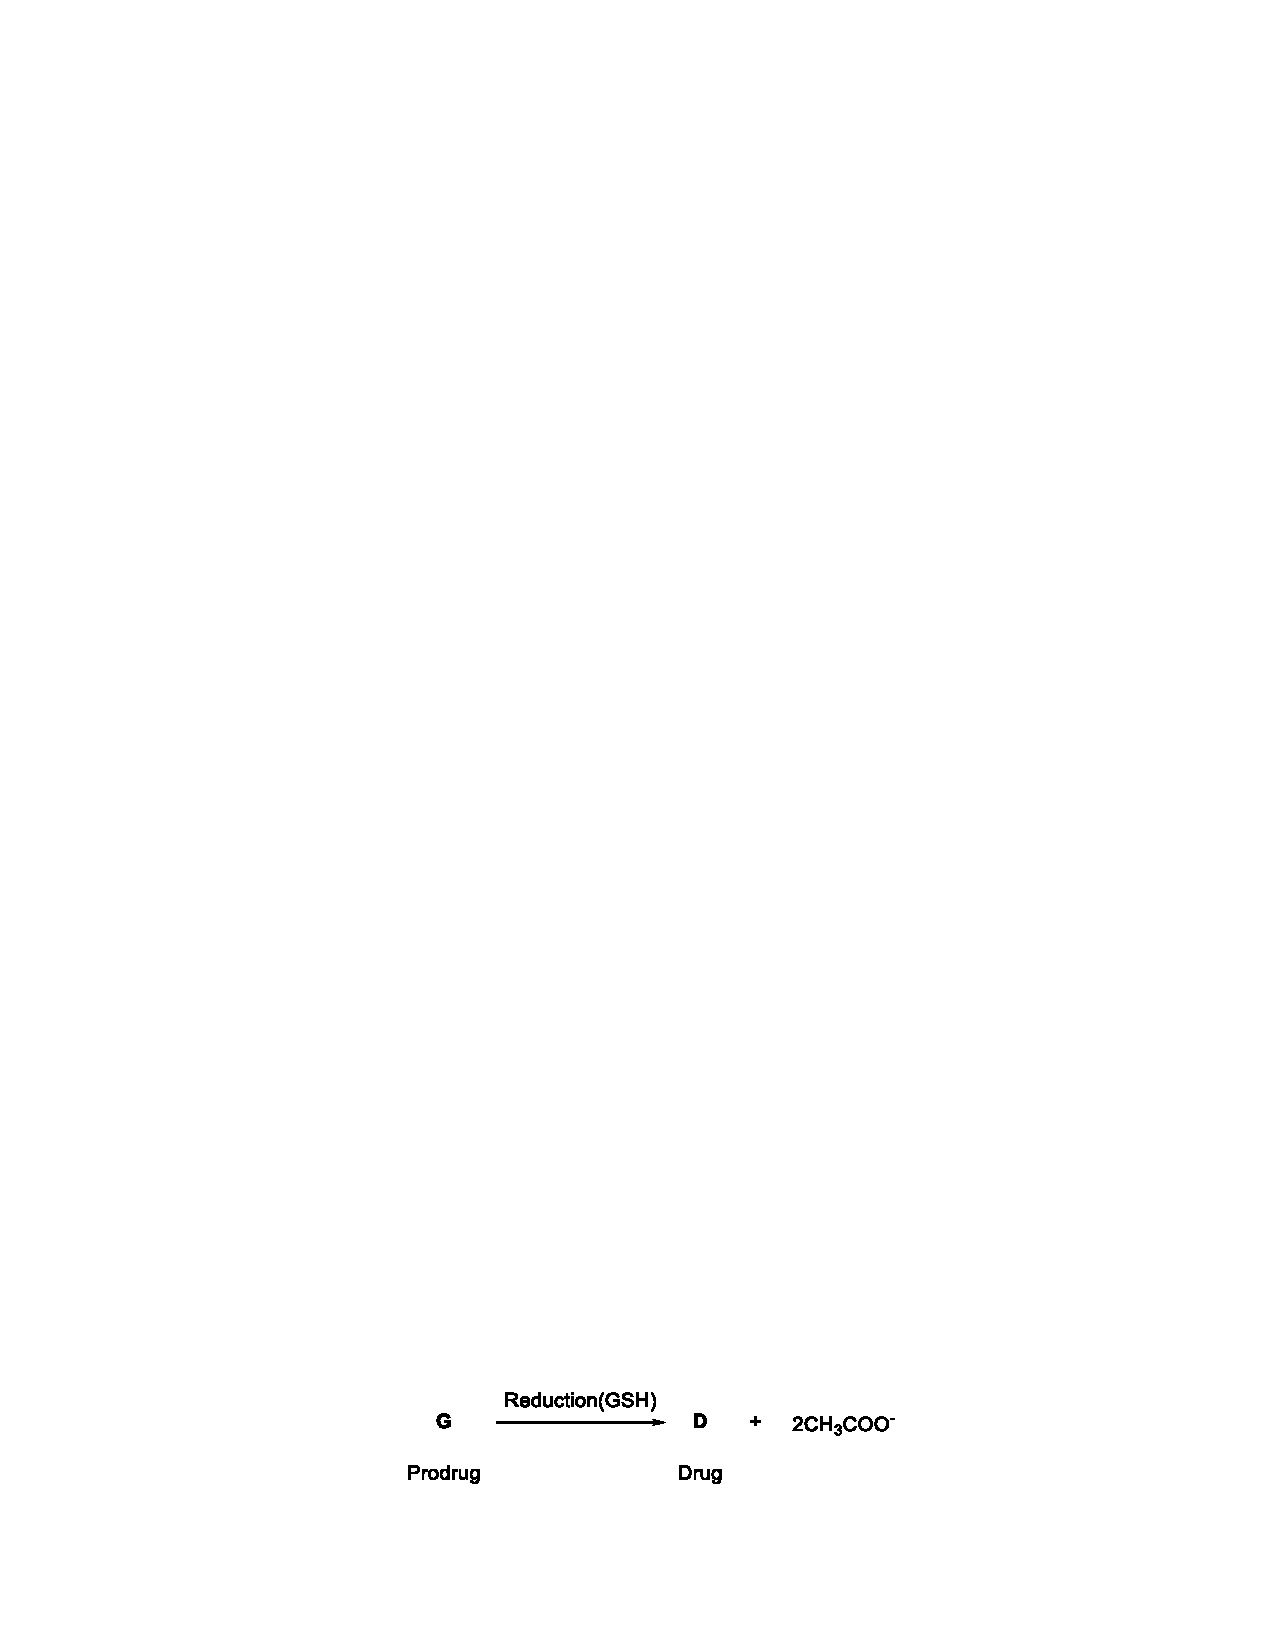
\includegraphics[width=8cm]{./pic/t14-6.pdf}
\end{figure}

\noindent\textbf{14.10.} 画出\textbf{G}的分子结构

\noindent\textbf{14.11.} 画出\textbf{G}中金属离子的\textit{d}轨道分裂并写出电子排布。

\noindent\textbf{14.12.} \textbf{G}是顺磁性还是反磁性的?

络合物\textbf{G}结晶成单斜晶体,其晶胞参数为:$a=14.9973$,$b=8.57220$,$c=11.1352$ \AA,$\beta=126.7690^{\circ} $,晶胞中的分子数$Z=4$,$M=436.16\ $g mol\textsuperscript{−1}(配合物在晶体结构中有一个水分子)。

\noindent\textbf{14.13.} 计算化合物的密度$\rho$。提示:单斜晶胞的体积为$V=a\times b\times c\times \sin\beta$



\newpage
\mysection{第15题\  盐中的钠化合物}
土耳其的盐湖盆地对于保护生物多样性非常重要,根据国际标准被归类为湿地。它也是土耳其保有鸟类最多的湖泊之一。有鸟类85种,昆虫129种(其中4种是特有的),15种哺乳动物和38种特有的植物。该湖满足了土耳其约40\%的食盐需求(作为食用盐)。盐湖中的盐是由气象水排入地下并融化先前形成的盐穹顶,并沿构造线携带它们而形成的。盐湖中的盐生产是通过在阳光下蒸发湖水来完成的。我们利用太阳能通过池式系统制盐。

\begin{figure}[h]
	\centering
	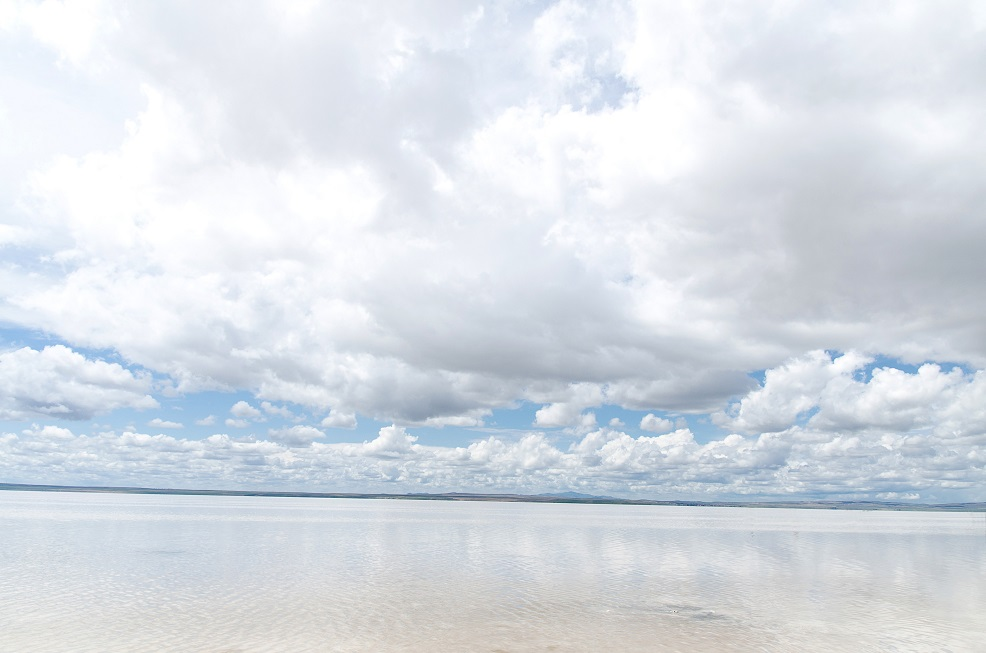
\includegraphics[width=10cm]{./pic/t15-1.jpg}
	\caption*{盐湖}
\end{figure}

食用盐是最常见的家用化学品之一。它是97\%到99\%的氯化钠,它是化学式为NaCl的离子化合物,代表钠和氯离子的比例为1:1。NaCl是最影响海水和许多多细胞生物体细胞外液盐度的化合物。食用盐的可食用形式通常用作调味品和食品防腐剂。钠的第二个主要应用是在亚冰冻天气中,用氯化物给道路除冰。大量氯化钠还用于许多工业过程中,例如氯碱工业和纯碱工业以及其他工业用途:水软化,医药,农业,消防和清洁剂。NaCl直接或间接用于生产许多钠化合物。世界上大部分产量都为钠化合物。下图显示了从NaCl制备一些钠化合物的方法。

\begin{figure}[h]
	\centering
	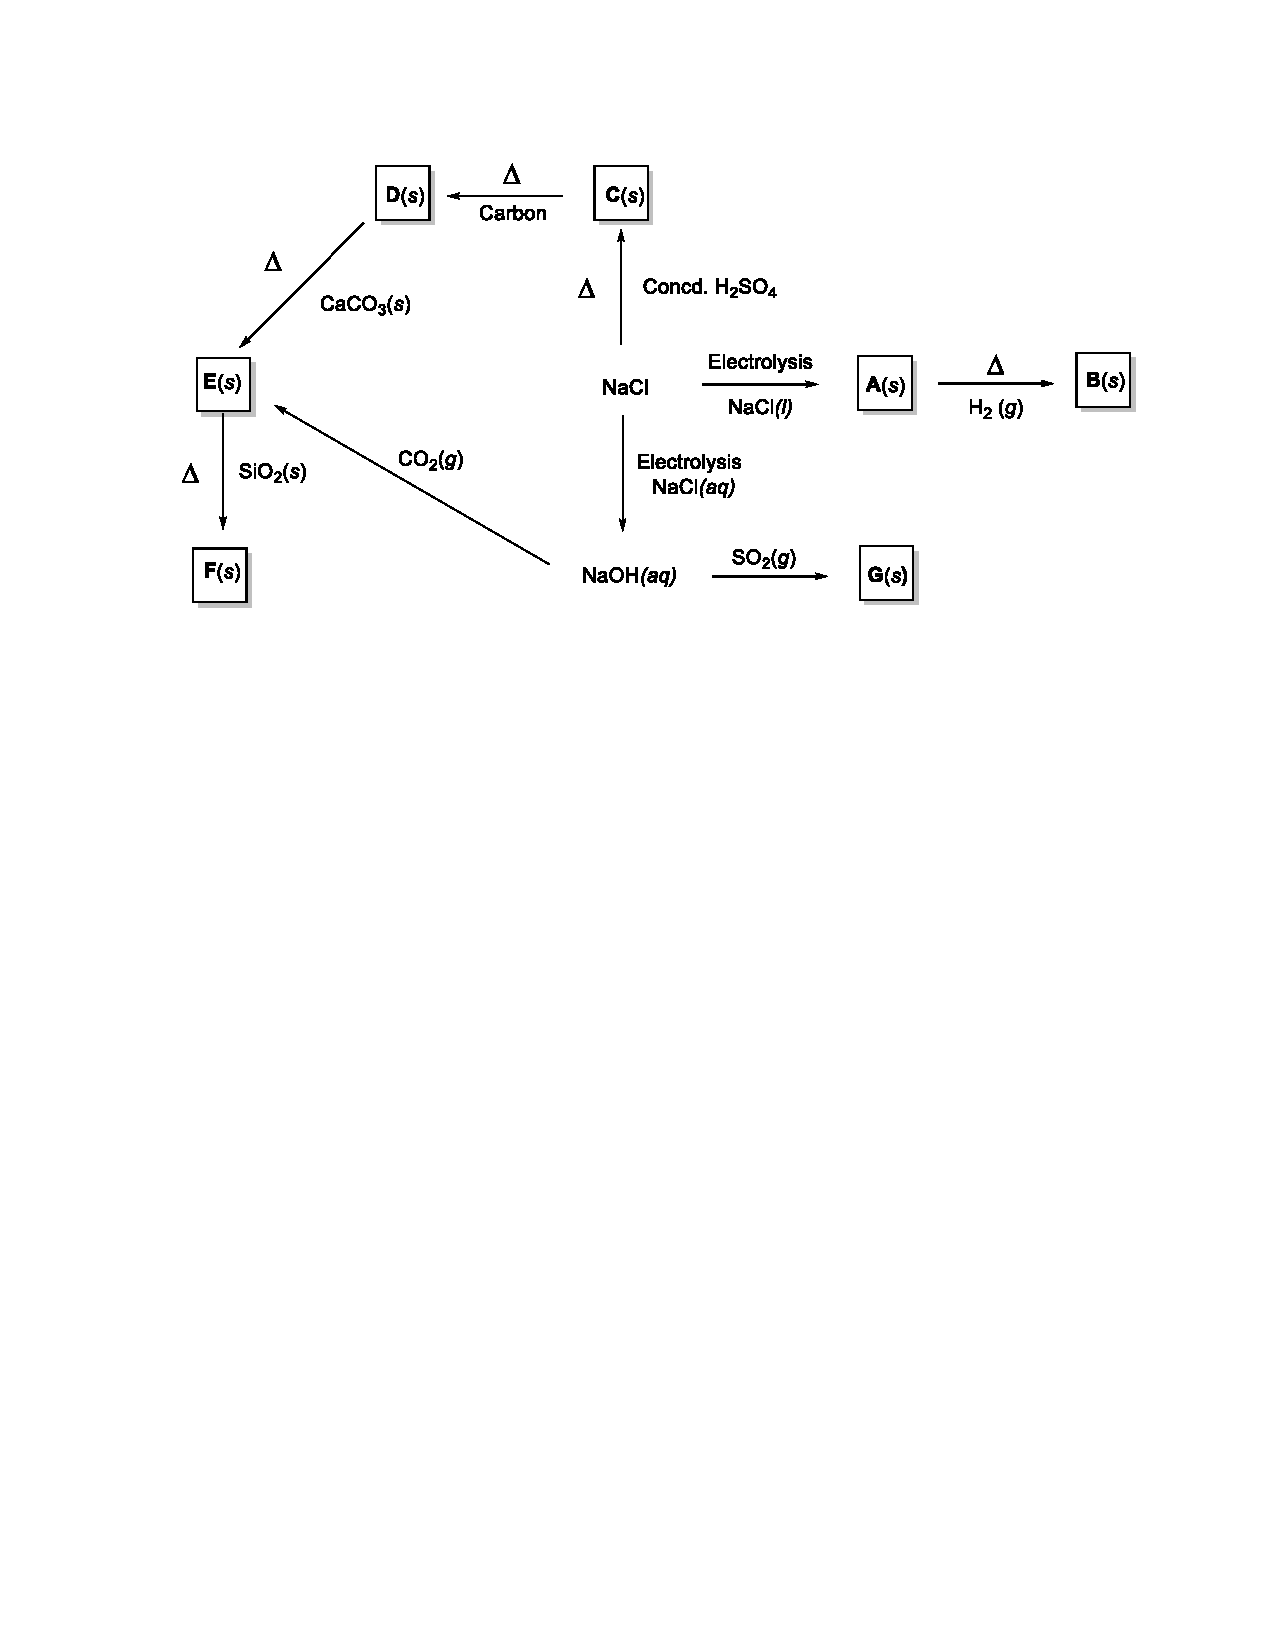
\includegraphics[width=14cm]{./pic/t15-2.pdf}
	\caption*{从NaCl开始制备一些钠化合物。}
\end{figure}

\noindent\textbf{15.1.} 写出\textbf{A}-\textbf{G}的分子式

碳酸钠(Na\textsubscript{2}CO\textsubscript{3},苏打粉),主要用于制造玻璃。它主要来源于天然产物,例如天然碱,Na\textsubscript{2}CO\textsubscript{3}·NaHCO\textsubscript{3}·$n$H\textsubscript{2}O。其主要可通过NaCl,CaCO\textsubscript{3},NH\textsubscript{3}用一个比利时化学家Ernest Solvay在1863年发明的方法生产。关键步骤包括NH\textsubscript{3}(g)和CO\textsubscript{2}(g)在饱和NaCl(aq)中反应。在所有可能从混合物结晶的离子型化合物中(NaCl,NH\textsubscript{4}Cl,NaHCO\textsubscript{3},NH\textsubscript{4}HCO\textsubscript{3}),溶解度最小的是碳酸氢钠(NaHCO\textsubscript{3})。它通过过滤分离出来,然后通过加热转化为碳酸钠(Na\textsubscript{2}CO\textsubscript{3})。根据解释,

\noindent\textbf{15.2.} 配平下面的方程式

$\ce{NaCl(aq) + CO2(g) + NH3(g) + H2O ->}$

$\ce{2NaHCO3(s) ->[\Delta]}$

\noindent\textbf{15.3.}
使用CaCO\textsubscript{3}(石灰石),你怎样才能获得你想要的CO\textsubscript{2}气体来生产NaHCO\textsubscript{3}?

\noindent\textbf{15.4.}
写出CaCO\textsubscript{3}的包含所有共振式的Lewis结构,并标出每个原子的形式电荷。

\noindent\textbf{15.5.}
描述CO$_3^{2-}$的分子几何结构并提出中心原子合理的杂化方式。

\noindent\textbf{15.6.}
按照键长增长的顺序排列CO$_3^{2-}$,CO,CO\textsubscript{2}

NaCl结晶为面心立方(fcc)结构。NaCl的密度为2180
kg m\textsuperscript{−3},Na\textsuperscript{+}的离子半径为99pm。

\noindent\textbf{15.7.} 在晶胞中有多少原子?什么原子占据八面体空隙?

\noindent\textbf{15.8.}
计算NaCl的晶胞长度和Cl\textsuperscript{−}的离子半径(用pm)

碱金属与氧气快速反应,生成几种不同的离子型氧化物。在适当的条件下,通常通过仔细控制氧气,每种碱金属都能生成氧化物M\textsubscript{2}O。
锂与过量氧气反应生成\textbf{A}和少量的\textbf{B}。钠与过量的氧气反应生成大部分\textbf{C}和少量\textbf{D}。钾,铷和铯反应与过量的氧气形成\textbf{E},\textbf{F}和\textbf{G}。

\noindent\textbf{15.9.} \textbf{A}-\textbf{G}是哪些常见的金属氧化物?

\noindent\textbf{15.11.} 画出过氧和超氧离子的分子轨道能级图并比较它们的键长和能量。

当LiClO\textsubscript{4},NaClO\textsubscript{4}和KClO\textsubscript{4}从水溶液结晶时,它们可能包含或不包含称为结晶水的水分子作为固体结构的一部分,尽管没有简单的规则可以确定地预测离子在固态中是否保留其全部或部分水化球,具有高电荷密度的阳离子倾向于将其全部或部分水化球保留在固态中。当阳离子具有低电荷密度时,它们往往会失去其水合球;因此,它们倾向于形成无水盐。Li\textsuperscript{+},Na\textsuperscript{+}和K\textsuperscript{+}的离子半径分别为76 pm,102 pm和138 pm。

\noindent\textbf{15.12.} 计算这些离子的电荷密度(单位用C mm\textsuperscript{−3})

\noindent\textbf{15.13.} 哪种高氯酸盐最易形成无水化合物?


\newpage
\mysection{第25题\  分光光度法测定抗组胺药}

分光光度法是用于确定药物分子的简单,快速和准确的方法。该方法基于两种试剂之间形成复合物。许多复合物是有色的,并在可见光区域有吸收。因此可以用分光光度法测定它们。

抗组胺药物\textbf{D}作为给电子基团,与$\pi$-受体\textbf{S}复合。所得的复合物在最大吸收(460 nm)处记录的吸光度与药物浓度线性相关,具有良好的相关系数。
$$
\begin{aligned}
\mathrm D+\mathrm S\rightleftharpoons\mathrm {DS}\\
K=\frac{[\mathrm{DS}]}{[\mathrm D][\mathrm S]}\\
\end{aligned}
$$
其中\([\mathrm{DS}]\),\([\mathrm D]\)与\([\mathrm S]\)分别代表\textbf{DS}复合物,\textbf{D}与\textbf{S}的平衡浓度。
\[
c_{\mathrm D}=[\mathrm D]+[\mathrm {DS}]
\] 
其中\(c_{\mathrm D}\)是药物的总浓度。

只有所形成的\textbf{DS}络合物可以吸收光的波长下,以下表达式成立:

 \[
A=\varepsilon_{\mathrm{DS}}l[\mathrm{DS}]
\] 
其中\(l\)是吸收池长度。

可以使用Benesi--Hildebrand方程来计算络合物的结合平衡常数,该方程取决于实验条件,其中一种组分应大量过量,以使其浓度不会随复合物的形成而改变。

\[
\frac{c_{\mathrm D}}{A_{\mathrm{DS}}}=\frac{1}{\varepsilon_{\mathrm{DS}}}+\frac{1}{\varepsilon_{\mathrm{DS}}K}\times\frac{1}{c_{\mathrm S}}
\]
其中\(c_{\mathrm S}\)与\(c_{\mathrm D}\)是\textbf{S}与\textbf{D}的总浓度。\(A_{\mathrm{DS}}\)是复合物的吸光度,\(\varepsilon_{\mathrm{DS}}\)是复合物的摩尔吸光系数,\(K\)是平衡常数。

\begin{figure}[h]
	\centering
	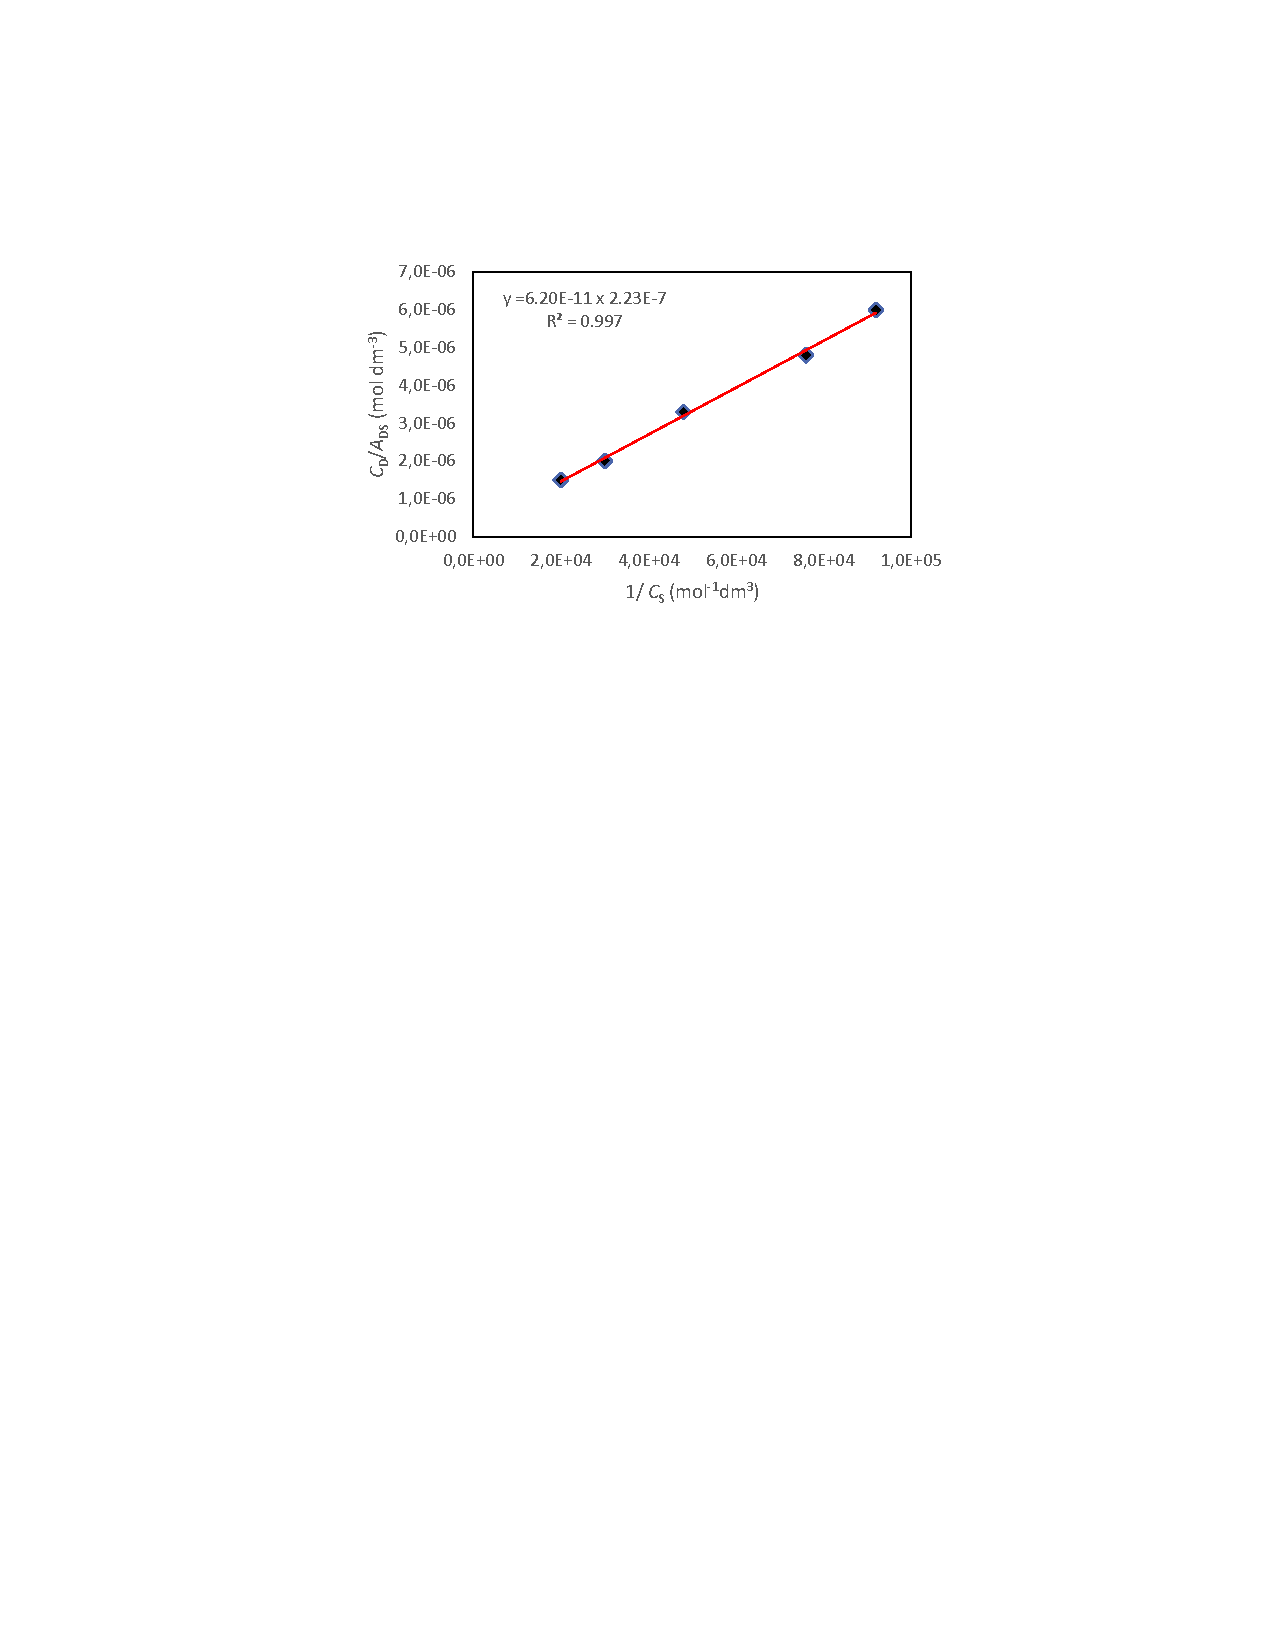
\includegraphics[width=12cm]{./pic/t25-1.pdf}
\end{figure}

\noindent\textbf{25.1.} 考虑在25
°C下记录的Benesi--Hildebrand图,给出复合物生成的平衡常数和复合物的摩尔吸光系数。


\noindent\textbf{25.2.}
\textbf{D}与\textbf{S}的起始浓度是9×10\textsuperscript{−5} mol
L\textsuperscript{−1},计算平衡时复合物形成的百分数。\textbf{D}与\textbf{S}在复合的时候比例为1:1。

\noindent\textbf{25.3.} 计算25 °C下的\(\Delta_rG^\ominus\),单位为kJ
mol\textsuperscript{−1}。

通过改变温度(25、45和60 °C)研究\textbf{D}与\textbf{S}的络合动力学。该表给出了在不同温度下的络合速率常数。

\begin{longtable}[]{@{}llll@{}}
	\toprule
	$T$ (°C) &25&45&60 \tabularnewline
	$k$ (min\textsuperscript{--1}) & 0.0200 &0.0504&0.0944\tabularnewline
	\bottomrule
\end{longtable}

\noindent\textbf{25.4.} 计算活化能\(E_a\)。

\noindent\textbf{25.5.}
已知\(k_{\mathrm{TST}}=\frac{k_{\mathrm BT}}{h}e^{-\frac{\Delta G^\ddag}{RT}}\),计算25 °C下的活化焓\(\Delta H^\ddag\),活化熵\(\Delta S^\ddag\)以及活化自由能\(\Delta G^\ddag\)。
(译注:原文为自由活化焓\(\Delta G^\ddag\))



\mychapter{实验试题}


\end{document}                          % The required last line